%%%%%%%%%%%%%%%%%%%%%%%%%%%%%%%%%%%%%%%%%%%%%%%%%%%%%%%%
% 							                           
%%%%%%%%%%%%%%%%%%%%%%%%%%%%%%%%%%%%%%%%%%%%%%%%%%%%%%%%

\documentclass[a4,12pt]{article}

%--- Generic packages ---%

\usepackage[english]{babel}
\usepackage[utf8]{inputenc}
\usepackage[T1]{fontenc}
\usepackage[babel=true]{csquotes}
\usepackage{amsmath}
\usepackage{amssymb}
\usepackage{float}
\usepackage{graphicx}
\usepackage{hyperref}

%--- Page structure ---%

\usepackage{fancyheadings}

\topmargin -1.5 cm
\oddsidemargin -0.5 cm
\evensidemargin -0.5 cm
\textwidth 17 cm
\setlength{\headwidth}{\textwidth}
\textheight 24 cm
\pagestyle{fancy}
\lhead[\fancyplain{}{\thepage}]{\fancyplain{}{\sl Rendering Introduction}}
\chead[\fancyplain{}{{\sl }}]{\fancyplain{}{{Lab Report}}}
\rhead[\fancyplain{}{}]{\fancyplain{}{Kylian Vincent}}
\lfoot{\fancyplain{}{}}
\cfoot{\fancyplain{}{}}
\cfoot{\thepage }
\rfoot{\fancyplain{}{}}

%--- Coding zone style ---%

\usepackage{tikz}
\usetikzlibrary{calc}
\usepackage[framemethod=tikz]{mdframed}
\usepackage{listings}             
\usepackage{textcomp}
%% For C++ code inclusion
\usepackage{xcolor}

\lstset{upquote=true,
	columns=flexible,
	keepspaces=true,
	breaklines,
	breakindent=0pt,
	alsoletter=\),
}

\lstset{classoffset=0,
	keywordstyle=\color{violet!75},
	deletekeywords={zeros,disp},
	classoffset=1,
	keywordstyle=\color{cyan},
	morekeywords={zeros,disp},
}

%% For C++ code inclusion
\lstset { %
	language=C++,
	backgroundcolor=\color{black!5}, % set backgroundcolor
}

\lstset{language=C++,
	basicstyle=\footnotesize,% basic font setting
	keywordstyle=\color{blue}\ttfamily,
	stringstyle=\color{red}\ttfamily,
	numbers=left, % display line numbers on the left
	commentstyle=\color{green!60!gray}\ttfamily,
	showstringspaces=false, % don't mark spaces in strings
	morecomment=[l][\color{magenta}]{\#}
}
\lstset{extendedchars=true,
	literate={0}{{\color{brown!65!black}0}}1 
	{1}{{\color{brown!65!black}1}}1 
	{2}{{\color{brown!65!black}2}}1 
	{3}{{\color{brown!65!black}3}}1 
	{4}{{\color{brown!65!black}4}}1 
	{5}{{\color{brown!65!black}5}}1 
	{6}{{\color{brown!65!black}6}}1 
	{7}{{\color{brown!65!black}7}}1 
	{8}{{\color{brown!65!black}8}}1 
	{9}{{\color{brown!65!black}9}}1 
	{(}{{\color{blue!50}(}}1 
	{)}{{\color{blue!50})}}1 
	{[}{{\color{blue!50}[}}1 
	{]}{{\color{blue!50}]}}1
	{-}{{\color{black}\textbf{-}}}1
	{+}{{\color{black}\textbf{+}}}1
	{=}{{\color{black}\textbf{=}}}1
	{:}{{\color{orange!50!yellow}:}}1
	{é}{{\'e}}1 
	{è}{{\`e}}1 
	{à}{{\`a}}1 
	{ç}{{\c{c}}}1 
	{œ}{{\oe}}1 
	{ù}{{\`u}}1
	{É}{{\'E}}1 
	{È}{{\`E}}1 
	{À}{{\`A}}1 
	{Ç}{{\c{C}}}1 
	{Œ}{{\OE}}1 
	{Ê}{{\^E}}1
	{ê}{{\^e}}1 
	{î}{{\^i}}1 
	{ô}{{\^o}}1 
	{û}{{\^u}}1 
}


%--- Math shortcuts ---%

\newcommand{\R}{\mathbb{R}}
\newcommand{\N}{\mathbb{N}}
\newcommand{\A}{\mathbf{A}}
\newcommand{\B}{\mathbf{B}}
\newcommand{\C}{\mathbf{C}}
\newcommand{\D}{\mathbf{D}}
\newcommand{\ub}{\mathbf{u}}

%--- Correction ---%

\usepackage{framed}
\usepackage{ifthen}
\usepackage{comment}
\usepackage{graphicx}

\newcounter{Nbquestion}

\newcommand*\question{%
	\stepcounter{Nbquestion}%
	\textbf{Question \theNbquestion. }}

\definecolor{shadecolor}{gray}{0.80}

%--- Questions style ---%

\mdfsetup{leftmargin=12pt}
\mdfsetup{skipabove=\topskip,skipbelow=\topskip}

\tikzset{
	warningsymbol/.style={
		rectangle,draw=red,
		fill=white,scale=1,
		overlay}}
\global\mdfdefinestyle{exampledefault}{
	hidealllines=true,leftline=true,
	innerrightmargin=0.0em,
	innerleftmargin=0.3em,
	leftmargin=0.0em,
	linecolor=red,
	backgroundcolor=orange!20,
	middlelinewidth=4pt,
	innertopmargin=\topskip,
}

\global\mdfdefinestyle{answer}{
	hidealllines=true,leftline=true,
	innerrightmargin=0.0em,
	innerleftmargin=0.3em,
	leftmargin=0.0em,
	linecolor=green,
	backgroundcolor=white,
	middlelinewidth=4pt,
	innertopmargin=\topskip,
}

%%%%%%%%%%%%%%%%%%%%%%%%%%%%%%%%%%%%%%%%%%%%%%%%%%%%%%%%
% 							               HEADING       
%%%%%%%%%%%%%%%%%%%%%%%%%%%%%%%%%%%%%%%%%%%%%%%%%%%%%%%%

\title{\textbf{Rendering Introduction\\Lab report}}
\author{
	\begin{tabular}{c}
		\textsc{Kylian Vincent}\\
	\end{tabular}}   
\date{\small \today}

\makeatletter
\def\thetitle{\@title}
\def\theauthor{\@author}
\def\thedate{\@date}
\makeatother 

\usepackage{etoolbox}
\usepackage{titling}
\setlength{\droptitle}{-7em}

\setlength{\parindent}{1cm}

\makeatletter
% bug patch about closing parenthesis from http://tex.stackexchange.com/q/69472
\patchcmd{\lsthk@SelectCharTable}{%
	\lst@ifbreaklines\lst@Def{`)}{\lst@breakProcessOther)}\fi}{}{}{}

%%%%%%%%%%%%%%%%%%%%%%%%%%%%%%%%%%%%%%%%%%%%%%%%%%%%%%%%
% 							DOCUMENT          
%%%%%%%%%%%%%%%%%%%%%%%%%%%%%%%%%%%%%%%%%%%%%%%%%%%%%%%%

\begin{document}
	\maketitle

	\tableofcontents
	\pagebreak
	
	%%%%%%%%%%%%%%%%%%%%%%%%%%%%%%%%%%%%%%%%%%%%%%%%%%%%%%%%
	% 						                  	PART 1
	%%%%%%%%%%%%%%%%%%%%%%%%%%%%%%%%%%%%%%%%%%%%%%%%%%%%%%%%
	\section{Worksheet 1}
	
	\subsection{Preview}
	\begin{center}
		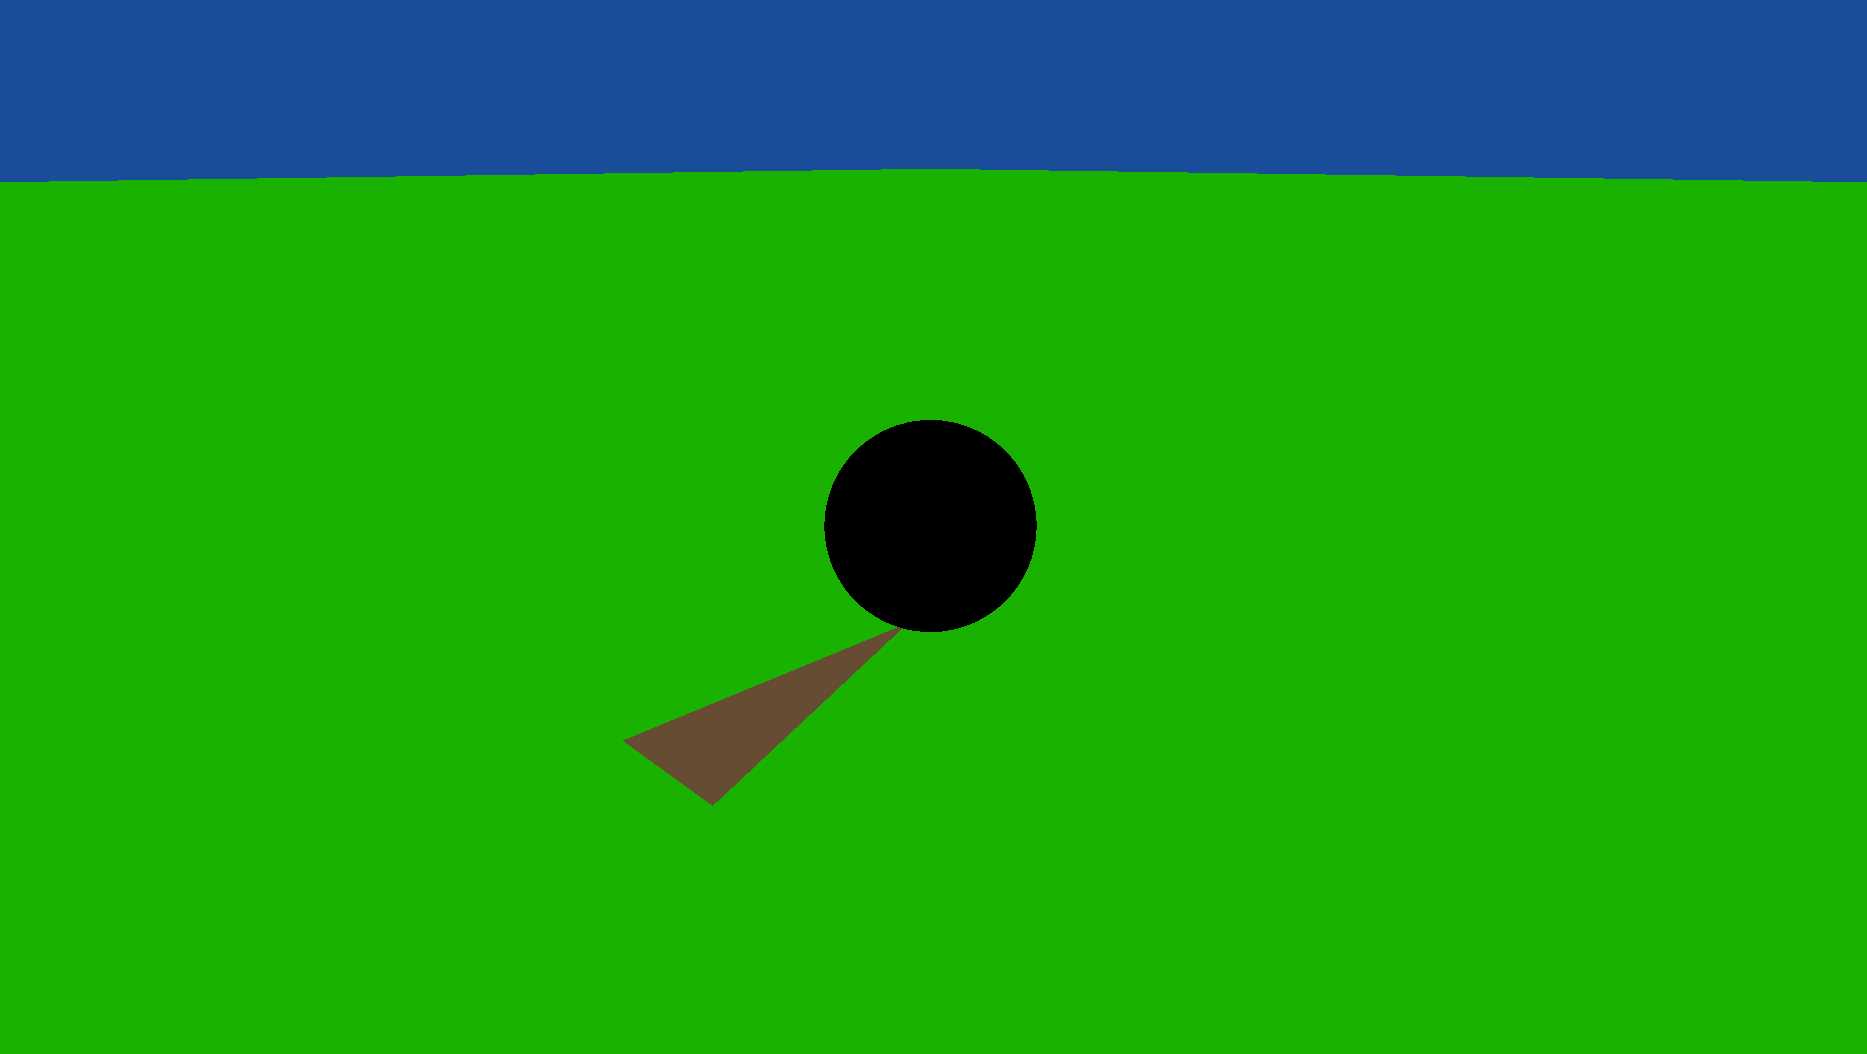
\includegraphics[width = 12cm]{./Worksheet1/Worksheet1_GettingStarted_Cropped.png}
	\end{center}
	
	\subsection{Rays generation}
	\textbf{RenderEngine.cpp}
	\begin{lstlisting}
		void RenderEngine::render()
		{
		cout << "Raytracing";
		Timer timer;
		timer.start();
		#pragma omp parallel for private(randomizer)
		for(int y = 0; y < static_cast<int>(res.y); ++y)
		{
			// Inner loop which runs through each pixel in a row and
			// stores the result of calling compute_pixel in the image array.
			for(int x = 0; x < static_cast<int>(res.x); x++)
			{
				image.at(y*res.y+x) = tracer.compute_pixel(x, y);
			}
		
			if(((y + 1) % 50) == 0) 
				cerr << ".";
			}
			timer.stop();
			cout << " - " << timer.get_time() << " secs " << endl;
		
			init_texture();
			done = true;
		}
	\end{lstlisting}
	
	\textbf{RayCaster.cpp}
	\begin{lstlisting}
		float3 RayCaster::compute_pixel(unsigned int x, unsigned int y) const
		{
			// Use the scene and its camera
			// to cast a ray that computes the color of the pixel at index (x, y).
			//
			// Input:  x, y        (pixel index)
			//
			// Return: Result of tracing a ray through the pixel at index (x, y)
			
			
			float3 result = make_float3(0.0f);
						
			float xip = x*win_to_ip.x + lower_left.x;
			float yip = y*win_to_ip.y + lower_left.y;
			float2 coords = make_float2(xip, yip);
			
			Ray r = scene->get_camera()->get_ray(coords);
			
			HitInfo hit = HitInfo();
			scene->closest_hit(r, hit);
			
			if (hit.has_hit) {
				result = get_shader(hit)->shade(r, hit);
			} else {
			result = get_background();
		}
		// Uncomment the following line to output a color using the ray direction 
		//return (r.direction + 1)/2;
		
		return result;
	}
	\end{lstlisting}
	
	\textbf{Camera.cpp}
	\begin{lstlisting}
	void Camera::set(const float3& eye_point, const float3& view_point, const float3& up_vector, float camera_constant)
	{
		// Compute camera coordinate frame (image plane normal and basis).
		eye = eye_point;
		lookat = view_point;
		up = up_vector;
		cam_const = camera_constant;
		
		ip_normal = normalize(lookat - eye);
		ip_xaxis = normalize(cross(ip_normal, up));
		ip_yaxis = cross(ip_xaxis, ip_normal);
		
		float film_height = 1;
		fov = 2*atan(film_height/(2*camera_constant)); //In radians
		fov *= 180*M_1_PIf; //In degrees
		//fov = 53.13f;
	}
	\end{lstlisting}
	
	\begin{lstlisting}
	/// Get direction of viewing ray from image coords.
	float3 Camera::get_ray_dir(const float2& coords) const
	{
		return normalize(ip_xaxis*coords.x + ip_yaxis*coords.y + ip_normal*cam_const);
	}
	\end{lstlisting}
	
	\begin{lstlisting}
	/// Return the ray corresponding to a set of image coords
	Ray Camera::get_ray(const float2& coords) const
	{
		return Ray(eye, get_ray_dir(coords), 0, 0);
	}
	\end{lstlisting}
	
	Below is a result of the output color computed using the ray directions :
	\begin{center}
		
\includegraphics[width =10cm]{./Worksheet1/ray_colors.png}
	\end{center}
	
	\subsection{Intersections}
	\textbf{Accelerator.cpp}
	\begin{lstlisting}
	bool Accelerator::closest_hit(optix::Ray& r, HitInfo& hit) const
	{
		// Loop through all the primitives to find the closest intersection (if any).
		closest_plane(r, hit);
		
		for (uint i = 0; i < primitives.size(); i++) {
			AccObj* obj = primitives[i];
			if (obj->geometry->intersect(r, hit, obj->prim_idx)) {
				r.tmax = hit.dist;
			}
		}
		
		return hit.has_hit;
	}
	\end{lstlisting}
	
	\textbf{Plane.cpp}
	\begin{lstlisting}
	bool Plane::intersect(const Ray& r, HitInfo& hit, unsigned int prim_idx) const
	{
		// Ray-plane intersection
		// Test if the plane intersects
		if (dot(r.direction, onb.m_normal) == 0) {
			// No intersection
			return false;
		}
		
		float dist = -(dot(r.origin, onb.m_normal) + d) / (dot(r.direction, onb.m_normal));
		
		// Check if t is in bounds
		if (dist < r.tmin) {
			return false;
		} else if (dist > r.tmax) {
			return false;
		}
	
		// Intersects with the plane, setting hit properties
		hit.has_hit = true;
		hit.dist = dist;
		hit.position = r.origin + r.direction*dist;
		hit.geometric_normal = onb.m_normal;
		hit.shading_normal = onb.m_normal;
		hit.material = &material;
		
		return true;
	}
	\end{lstlisting}
	
	\textbf{Triangle.cpp}
	\begin{lstlisting}
	bool intersect_triangle(const Ray& ray,
	const float3& v0,
	const float3& v1,
	const float3& v2,
	float3& n,
	float& t,
	float& v,
	float& w)
	{		
		// Test intersection with containing plane first
		float3 e0 = (v1 - v0);
		float3 e1 = (v0 - v2);
		n = cross(e0, e1);
		if (dot(ray.direction, n) == 0) {
			// No intersection
			return false;
		}
		
		float3 v0_minus_o = v0 - ray.origin;
		float denom = dot(ray.direction, n);
		t = dot(v0_minus_o, n) / denom;
		
		// Check if t is in bounds
		if (t < ray.tmin) {
			return false;
		} else if (t > ray.tmax) {
			return false;
		}
		
		// Vector decomposition
		float3 num_denom = cross(v0_minus_o, ray.direction)/denom;
		v = dot(num_denom, e1);
		w = dot(num_denom, e0);
		
		n = -n;
		return (v >= 0 && w >= 0 && v + w <= 1);
	}
	
	
	bool Triangle::intersect(const Ray& r, HitInfo& hit, unsigned int prim_idx) const
	{
		// Ray-triangle intersection
		float dist, v, w;
		float3 normal;
		bool intersects = ::intersect_triangle(r, v0, v1, v2, normal, dist, v, w);
		
		if (intersects) {
			hit.has_hit = true;
			hit.dist = dist;
			hit.position = r.origin + r.direction*dist;
			hit.geometric_normal = normalize(normal);
			hit.shading_normal = hit.geometric_normal;
			hit.material = &material;
		}
		
		return intersects;
	}
	\end{lstlisting}
	
	\textbf{Sphere.cpp}
	\begin{lstlisting}
	bool Sphere::intersect(const Ray& r, HitInfo& hit, unsigned int prim_idx) const
	{
		float3 ray_to_sphere = r.origin - center;
		float b_half = dot(ray_to_sphere, r.direction);
		float c = dot(ray_to_sphere, ray_to_sphere) - pow(radius, 2);
		
		float discrim = pow(b_half, 2) - c;
		
		if (discrim < 0) {
			return false;
		}
		float t1 = -b_half - sqrt(discrim);
		float t2 = -b_half + sqrt(discrim);
		float dist;
		if (t1 > r.tmin && t1 < r.tmax) {
			dist = t1;
		} else if (t2 > r.tmin && t2 < r.tmax) {
			dist = t2;
		} else {
			// None of the distances are in bounds: no intersection
			return false;
		}
		
		hit.has_hit = true;
		hit.dist = dist;
		hit.position = r.origin + r.direction*dist;
		hit.geometric_normal = normalize(hit.position - center);
		hit.shading_normal = hit.geometric_normal;
		hit.material = &material;
		
		return true;
	}
	\end{lstlisting}
	\begin{center}
	\begin{minipage}[b]{0.40\linewidth}
		\begin{center}
			
\includegraphics[width =\textwidth]{./Worksheet1/blue_closest_hit.png}\\
			\textit{No intersection implemented : only blue background}
		\end{center}
	\end{minipage}
	\hspace{0.05\linewidth}
	\begin{minipage}[b]{0.40\linewidth}
		\begin{center}
			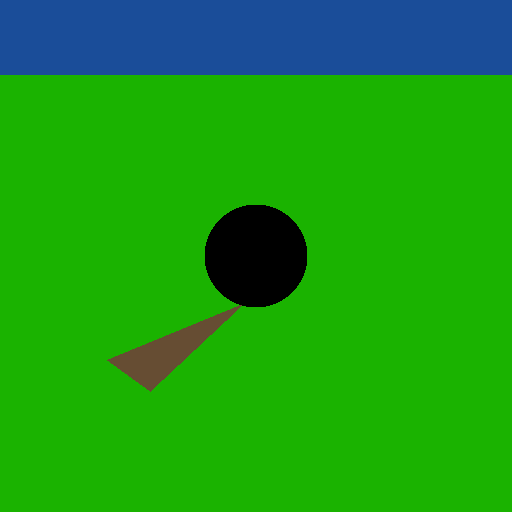
\includegraphics[width =\textwidth]{./Worksheet1/intersection.png}\\
			\textit{Every intersection implemented : identical to preview}
		\end{center}
	\end{minipage}
	\end{center}

	Implementation of the Lambertian in \textbf{Lambertian.cpp} :
	\begin{lstlisting}
	float3 Lambertian::shade(const Ray& r, HitInfo& hit, bool emit) const
	{
		float3 rho_d = get_diffuse(hit);
		float3 result = make_float3(0.0f);
		
		for (int i = 0; i < lights.size(); i++) {
			Light* light = lights[i];
			float3 dir, Li;
			if (light->sample(hit.position, dir, Li)) {
				float cosine = dot(dir, hit.shading_normal)/(length(dir) + length(hit.shading_normal));
				if (cosine > 0) {
					result += cosine * Li;
				}
			}
			
		}
		
		return result*rho_d + Emission::shade(r, hit, emit);
	}
	\end{lstlisting}
	
	%%%%%%%%%%%%%%%%%%%%%%%%%%%%%%%%%%%%%%%%%%%%%%%%%%%%%%%%
	% 						                  	PART 2
	%%%%%%%%%%%%%%%%%%%%%%%%%%%%%%%%%%%%%%%%%%%%%%%%%%%%%%%%
	\section{Worksheet 2}
	
	\subsection{Shading of diffuse objects}
	\textbf{PointLight.cpp}
	\begin{lstlisting}
	bool PointLight::sample(const float3& pos, float3& dir, float3& L) const
	{
		if (!shadows) {
		return true;
		}
		
		// Test if there's a hit before the object
		dir = light_pos - pos;
		float dist = length(dir);
		dir = normalize(dir);
		
		// Light fading
		L = intensity/(pow(dist, 2));
		
		Ray shadow_ray = Ray(light_pos, -dir, 0, 0, dist - 1e-4);
		HitInfo hit;
		
		return !tracer->trace_to_any(shadow_ray, hit);
	}
	\end{lstlisting}
	
	\begin{center}
		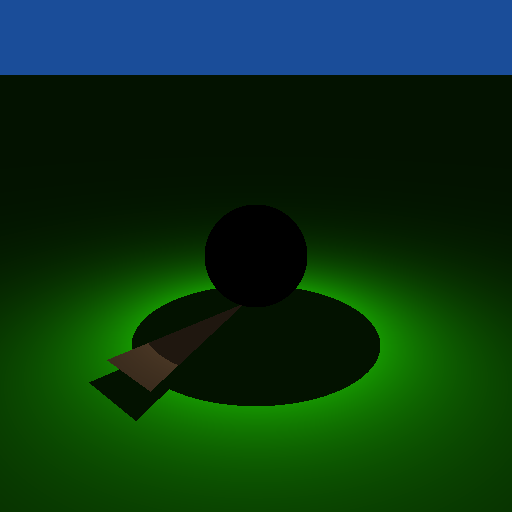
\includegraphics[width =8cm]{./Worksheet2/hard_shadows.png}\\
		\textit{Hard shadows}
	\end{center}
	
	The computation of the ray-triangle intersection is done with an inverted normal for the triangle (the triangle is facing down). In order to display correctly the triangle color its normal has to be inverted.
	
	\subsection{Reflection and refraction}
	\textbf{RayTracer.cpp}
	\begin{lstlisting}
	bool RayTracer::trace_reflected(const Ray& in, const HitInfo& in_hit, Ray& out, HitInfo& out_hit) const
	{
		out.direction = optix::reflect(in.direction, in_hit.shading_normal);
		out.origin = in_hit.position;
		out.ray_type = 0;
		out.tmax = RT_DEFAULT_MAX;
		out.tmin = 1.0e-4f;
		
		out_hit.ray_ior = in_hit.ray_ior;
		out_hit.trace_depth = in_hit.trace_depth + 1;
		
		return trace_to_closest(out, out_hit);
	}
	\end{lstlisting}
	
	\begin{lstlisting}
	bool RayTracer::trace_refracted(const Ray& in, const HitInfo& in_hit, Ray& out, HitInfo& out_hit) const {
		float3 normal;
		float cos_theta_in;
		out_hit.ray_ior = get_ior_out(in, in_hit, out.direction, normal, cos_theta_in);
		out_hit.trace_depth = in_hit.trace_depth + 1;
		
		bool is_refracted = optix::refract(out.direction, in.direction, normal, out_hit.ray_ior/in_hit.ray_ior);
		if (!is_refracted) {
			// Fully reflected so we call the reflexion for the refractive part
			return trace_reflected(in, in_hit, out, out_hit);
		}
		
		out.origin = in_hit.position;
		out.ray_type = 0;
		out.tmax = RT_DEFAULT_MAX;
		out.tmin = 1.0e-4f;
		
		return trace_to_closest(out, out_hit);
	}
	\end{lstlisting}
	
	The function \textit{get\_ior\_out} eases finding the index of refraction of the outside material (explanation of the function in comments):
	\begin{lstlisting}
	float RayTracer::get_ior_out(const Ray& in, const HitInfo& in_hit, float3& dir, float3& normal, float& cos_theta_in) const
	{
		// Get the refractive index of the material is which the ray is entering by refraction, only support interfaces
		// air/material or material/air.
		// If getting out of a material (detected because the normal is pointing to the outside) the refractive index is
		// automatically set to 1.0f
		// Sets normal and cos_theta_in according to the ray and hit_info
		normal = in_hit.shading_normal;
		dir = -in.direction;
		cos_theta_in = dot(normal, dir);
		if(cos_theta_in < 0.0)
		{
			normal = -normal;
			cos_theta_in = -cos_theta_in;
			return 1.0f;
		}
		const ObjMaterial* m = in_hit.material;
		return m ? m->ior : 1.0f;
	}
	\end{lstlisting}
	
	
	\begin{center}
		\begin{minipage}[b]{0.40\linewidth}
			\begin{center}
				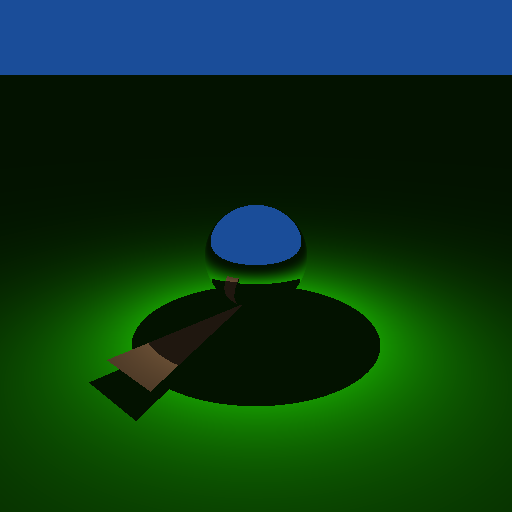
\includegraphics[width =\textwidth]{./Worksheet2/mirror_ball.png}\\
				\textit{Mirror material : 100\% reflection\vspace{1em}}
			\end{center}
		\end{minipage}
		\hspace{0.05\linewidth}
		\begin{minipage}[b]{0.40\linewidth}
			\begin{center}
				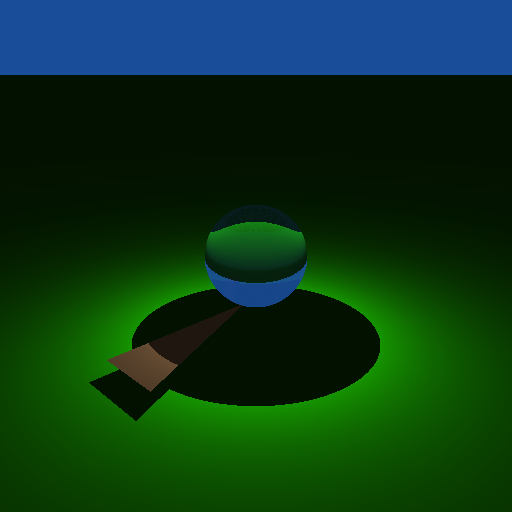
\includegraphics[width =\textwidth]{./Worksheet2/transparent_ball.png}\\
				\textit{Transparent material : 90\% refraction, \%10 reflection}
			\end{center}
		\end{minipage}
	\end{center}
	
	For the mirror-material rendering i'm not sure of the output, it seems like a lot of refraction more than transparency, should it be that way or did I make a mistake ?
	
	\subsection{Adding the corrected Phong Model}
	In order to obtain the glossy material we have to include Phong Model computation to add specular and diffuse characteristics to objects.
	
	\textbf{Phong.cpp}
	
	\begin{lstlisting}
	float3 Phong::shade(const Ray& r, HitInfo& hit, bool emit) const
	{
		float3 rho_d = get_diffuse(hit);
		float3 rho_s = get_specular(hit);
		float s = get_shininess(hit);
		float3 wi, wo, wr, Li;
		float3 Lr = make_float3(0.0);
		
		for (int i = 0; i < lights.size(); i++) {
			Light *light = lights[i];
			if (light->sample(hit.position, wi, Li)) {
				// Not in shadows, we add this light participation
				wr = normalize(reflect(-wi, hit.shading_normal));
				wo = normalize(-r.direction);
				
				// Compute phong for this light
				Li = make_float3(fmax(dot(wi, hit.shading_normal), 0));
				
				float3 first_coeff = rho_d*M_1_PIf;
				float dotproduct = dot(wo, wr);
				dotproduct = fmax(dotproduct, 0);
				float3 second_coeff = rho_s*(s + 2)*pow(dotproduct, s)*M_1_PIf/2;
				
				Li *= (first_coeff + second_coeff);
				Lr += Li;
			}
		}
		return Lr + Lambertian::shade(r, hit, emit);
	}
	\end{lstlisting}
	
	\textbf{Glossy.cpp}
	\begin{lstlisting}
	float3 Glossy::shade(const Ray& r, HitInfo& hit, bool emit) const
	{
		if(hit.trace_depth >= max_depth)
			return make_float3(0.0f);
		
		float R;
		Ray reflected, refracted;
		HitInfo hit_reflected, hit_refracted;
		tracer->trace_reflected(r, hit, reflected, hit_reflected);
		tracer->trace_refracted(r, hit, refracted, hit_refracted, R);
		
		return R*shade_new_ray(reflected, hit_reflected) + (1.0f - R)*shade_new_ray(refracted, hit_refracted) + Phong::shade(r, hit, emit);
	}
	\end{lstlisting}
	
	The Glossy shader creates a reflected ans refracted ray and mix their results according to the coefficient R between more reflection or refraction (linear combination). A Phong model component is added to render the specular and diffusive aspect of the material.\\
	
	Thus we see the light reflexion on the ball :
	
	\begin{center}
		\begin{minipage}[b]{0.40\linewidth}
			\begin{center}
				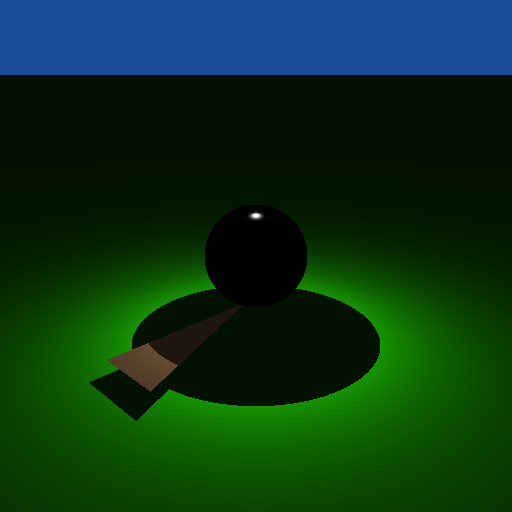
\includegraphics[width =\textwidth]{./Worksheet2/phong_cor.png}\\
				\textit{Phong Model with specular and diffuse components}
			\end{center}
		\end{minipage}
		\hspace{0.05\linewidth}
		\begin{minipage}[b]{0.40\linewidth}
			\begin{center}
				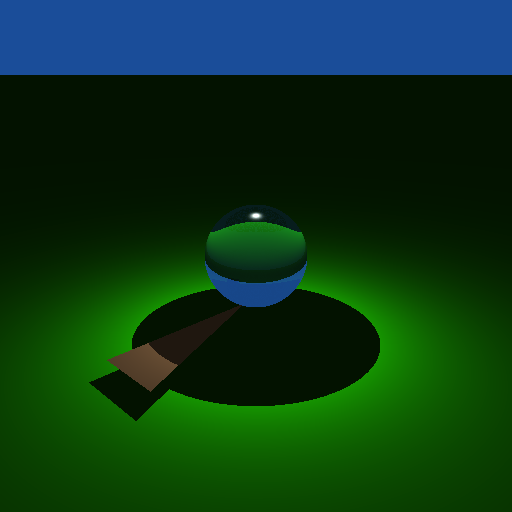
\includegraphics[width =\textwidth]{./Worksheet2/glossy_cor.png}\\
				\textit{Glossy material : Transparent material with Phong Model}
			\end{center}
		\end{minipage}
	\end{center}
	%%%%%%%%%%%%%%%%%%%%%%%%%%%%%%%%%%%%%%%%%%%%%%%%%%%%%%%%
	% 						                  	PART 3
	%%%%%%%%%%%%%%%%%%%%%%%%%%%%%%%%%%%%%%%%%%%%%%%%%%%%%%%%
	\section{Worksheet 3}
	\subsection{Textures in the framework}
	In \textbf{RenderEngine.cpp} the texture file for the plane is loaded using this code in \textit{load\_files} : 
	\begin{lstlisting}
	 // Insert default scene
	 scene.add_plane(make_float3(0.0f, 0.0f, 0.0f), make_float3(0.0f, 1.0f, 0.0f), "../models/default_scene.mtl", 1, 0.2f); // last argument is texture scale
	 scene.add_sphere(make_float3(0.0f, 0.5f, 0.0f), 0.3f, "../models/default_scene.mtl", 2);
	 scene.add_triangle(make_float3(-0.2f, 0.1f, 0.9f), make_float3(0.2f, 0.1f, 0.9f), make_float3(-0.2f, 0.1f, -0.1f), "../models/default_scene.mtl", 3);
	 scene.add_light(new PointLight(&tracer, make_float3(M_PIf), make_float3(0.0f, 1.0f, 0.0f)));
	 cam.set(make_float3(2.0f, 1.5f, 2.0f), make_float3(0.0f, 0.5, 0.0f), make_float3(0.0f, 1.0f, 0.0f), 1.0f);
	\end{lstlisting}
	
	The file \textit{default\_scene.mtl} contains rendering constants and the filename of the texture to load.\\
		
		
	By looking at the file \textbf{Textured.cpp} we can see how the color are retrieved from the texture. The objects have two components, a diffuse and ambient (embedded in emission) component. For objects these two components are computed respectively by functions \textit{get\_diffuse} and \textit{get\_emission}.\\
	
	For the textured objects it's a bit different as the color has to take into account the texture color within the environment and object properties. To do so, the texture diffuse term is defined as the texture color (linearly interpolated from the texture using the hit coordinates). The emission term is a combination between ambient material properties, diffuse material properties and texture color interpolated.
	
	
%	In a rendering texture color are mapped onto a surface and then each rendered pixel find its corresponding value in the texture. This mapping can be either linear (\textit{sample\_linear}) or based on the nearest texel (\textit{sample\_nearest}). Then the color is retrieved from the texture image using the \textit{look\_up} function which load the corresponding color depending on the number of channels in the image (Grey levels, grey levels and transparency, RGB, RGB and transparency) :
%	
%	\begin{lstlisting}
%	float4 Texture::look_up(unsigned int idx) const
%	{
%		idx *= channels;
%		switch(channels)
%		{
%			case 1: 
%			{
%				float v = convert(data[idx]);
%				return make_float4(v, v, v, 1.0f);
%			}
%			case 2: 
%			return make_float4(convert(data[idx]), convert(data[idx]), convert(data[idx]), convert(data[idx + 1]));
%			case 3: 
%			return make_float4(convert(data[idx]), convert(data[idx + 1]), convert(data[idx + 2]), 1.0f);
%			case 4: 
%			return make_float4(convert(data[idx]), convert(data[idx + 1]), convert(data[idx + 2]), convert(data[idx + 3]));
%		}
%		return make_float4(0.0f);
%	}
%	\end{lstlisting}
	
	
	
	\subsection{Textures coordinates on a plane}
	\textbf{Plane.cpp}
	\begin{lstlisting}
	void Plane::get_uv(const float3& hit_pos, float& u, float& v) const
	{
		// Do an inverse mapping from hit position to texture coordinates.
		u = dot((hit_pos - position), onb.m_tangent) * tex_scale;
		v = dot((hit_pos - position), onb.m_binormal) * tex_scale;
	}
	\end{lstlisting}
	 In the function \textit{intersect} I added just before the return statement a test to set the texture coordinates :
	 \begin{lstlisting}
	 // Test for texture
	 if (material.has_texture) {
	 	get_uv(hit.position, hit.texcoord.x, hit.texcoord.y);
	 }
	 \end{lstlisting}
	 
	 We obtain the grass textures mapped on the plane and we can change this texture by a tileable one of our choice by changing the filename in the \textit{default\_scene.mtl} file :
	 \begin{center}
	 \begin{minipage}[b]{0.40\linewidth}
		 \begin{center}
		 	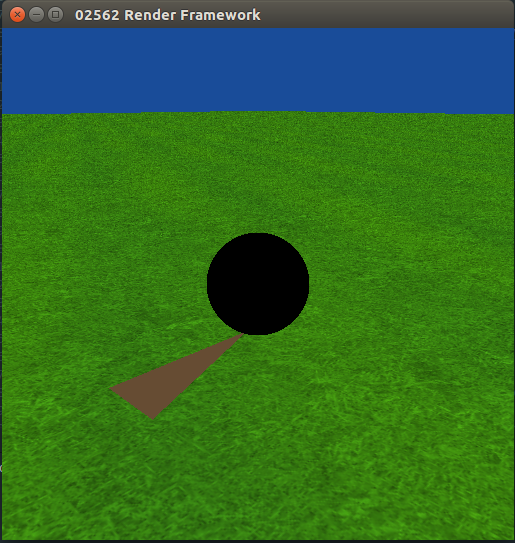
\includegraphics[width = \textwidth]{./Worksheet3/ScreenshotPreviewTexture.png}\\
		 	\textit{Preview of the grass texture}\\
		 	\hspace{1em}
		 \end{center}
	\end{minipage}
	\hspace{0.05\linewidth}
	\begin{minipage}[b]{0.40\linewidth}
		\begin{center}
			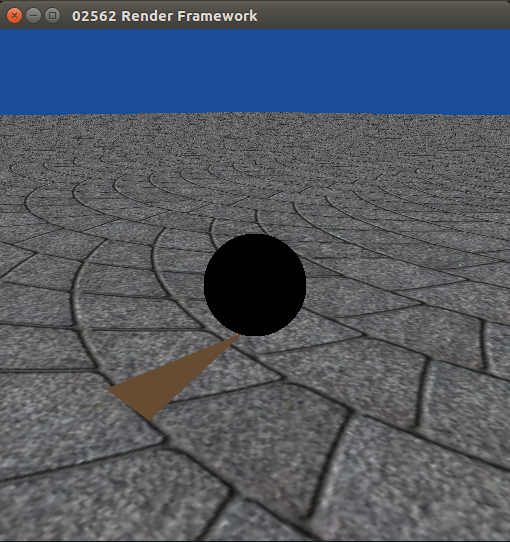
\includegraphics[width =\textwidth]{./Worksheet3/PavementPreview.png}\\
			\textit{Preview of a texture of a tileable pavement}
		\end{center}
	\end{minipage}
	\end{center}
	
	\subsection{Texture Lookup}
	\textbf{Texture.cpp}
	\begin{lstlisting}
	float4 Texture::sample_nearest(const float3& texcoord) const
	{
		if(!fdata)
		return make_float4(0.0f);
		
		double s, t, a, b;
		int U, V;
		s = texcoord.x - floor(texcoord.x);
		t = texcoord.y - floor(texcoord.y);
		// We revert vertical axis
		t = 1 - t;
		a = s * width;
		b = t * height;
		U = (int)(a + 0.5) % width;
		V = (int)(b + 0.5) % height;
		// We revert the vertical axis
		return fdata[U + V*width];
		//    return make_float4(0.0f);
	}
	\end{lstlisting}
	
	With this nearest texel computation we obtain the following results :
	
	\begin{center}
		\begin{minipage}[b]{0.40\linewidth}
			\begin{center}
				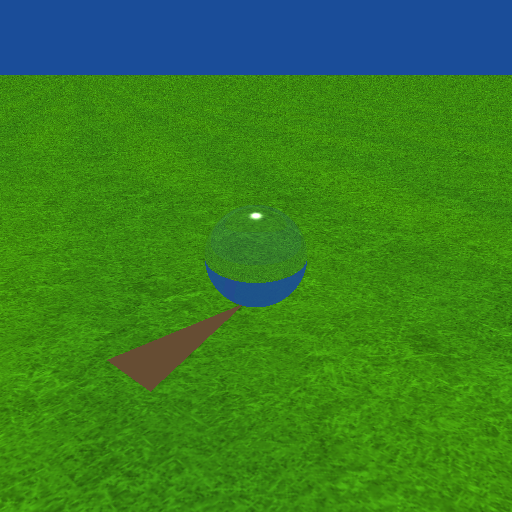
\includegraphics[width = \textwidth]{./Worksheet3/TexturesRenderingFlat.png}\\
				\textit{Rendering using base colours}\\
				\hspace{1em}
			\end{center}
		\end{minipage}
		\hspace{0.05\linewidth}
		\begin{minipage}[b]{0.40\linewidth}
			\begin{center}
				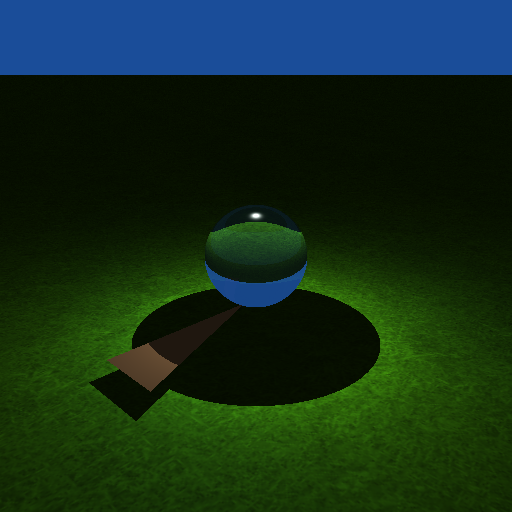
\includegraphics[width =\textwidth]{./Worksheet3/TexturesRenderingShadows.png}\\
				\textit{Rendering using the Lambertian Shader}
			\end{center}
		\end{minipage}
	\end{center}
	
	With the Lambertian shader we can then adapt the gamma to make the scene brighter :
	
	\begin{center}
		\begin{minipage}[b]{0.40\linewidth}
			\begin{center}
				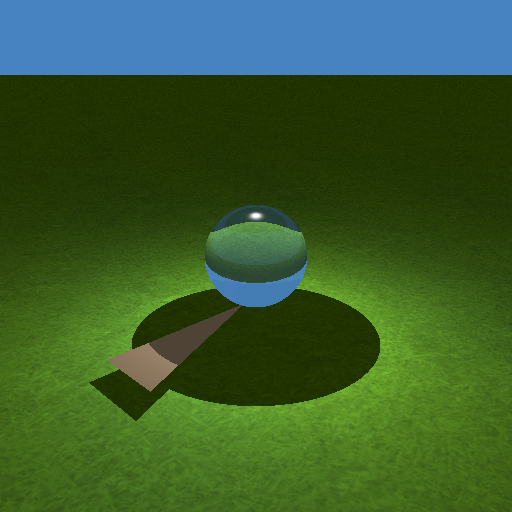
\includegraphics[width = \textwidth]{./Worksheet3/TexturesRenderingShadowsGamma.png}\\
				\textit{Lambertian rendering with gamma increased once}
			\end{center}
		\end{minipage}
		\hspace{0.05\linewidth}
		\begin{minipage}[b]{0.40\linewidth}
			\begin{center}
				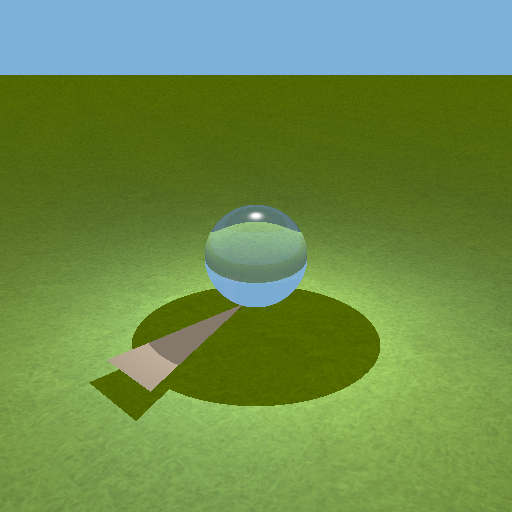
\includegraphics[width =\textwidth]{./Worksheet3/TexturesRenderingShadowsGammaGamma.png}\\
				\textit{Lambertian rendering with gamma increased twice (too much correction)}
			\end{center}
		\end{minipage}
	\end{center}
	
	Bilinear implementation :
	\begin{lstlisting}
	float4 Texture::sample_linear(const float3& texcoord) const
	{
	if(!fdata)
	return make_float4(0.0f);
	
	double s, t, a, b;
	int U, V;
	s = texcoord.x - floor(texcoord.x);
	t = texcoord.y - floor(texcoord.y);
	// We revert vertical axis
	t = 1 - t;
	a = s * width;
	b = t * height;
	U = (int)a;
	V = (int)b;
	
	float4 i_a, i_b, i_c, i_d;
	// We need a modulo when taking the U+1 or V+1 coordinate to make sure
	// we're not going outside the texture image
	i_a = fdata[U + V*width];
	i_b = fdata[(U+1)%height + V*width];
	i_c = fdata[U + ((V+1)%width)*width];
	i_d = fdata[(U+1)%height + ((V+1)%width)*width];
	
	return bilerp(i_a, i_b, i_c, i_d, a - U, b - V);
	}
	\end{lstlisting}
	
	Scaling the texture is done using the last argument of function \textbf{Scene}.\textit{add\_plane}. When this factor is lowered, then as the coordinates are scaled with this factor, the texture is magnified (larger).
	Scaling the textures with a too low scaling factor lead to magnification at the bottom part of our image. Indeed the texture image will cover a really wide unitary texture area and a texel will cover multiple pixels. The inverse phenomena produces aliasing in the far part of the plane.\\
	
	Here is an example of magnification when the texture image scaling factor is too low:
	
	\begin{center}
		\begin{minipage}[b]{0.40\linewidth}
			\begin{center}
				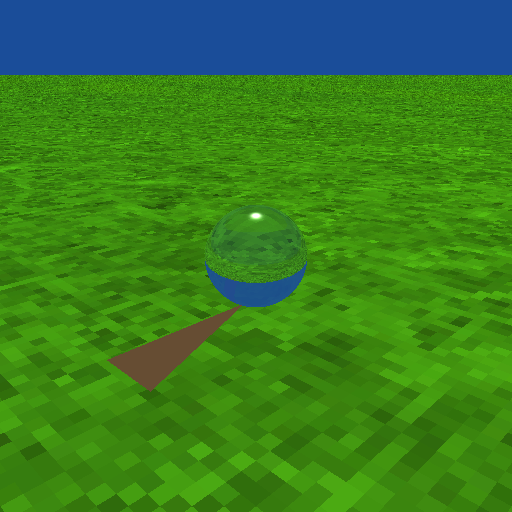
\includegraphics[width = \textwidth]{./Worksheet3/MagnifRenduNearest.png}\\
				\textit{Nearest sampling with a scaling factor divided by 10 (0.02 instead of 0.2)\\\vspace{1em}}
			\end{center}
		\end{minipage}
		\hspace{0.05\linewidth}
		\begin{minipage}[b]{0.40\linewidth}
			\begin{center}
				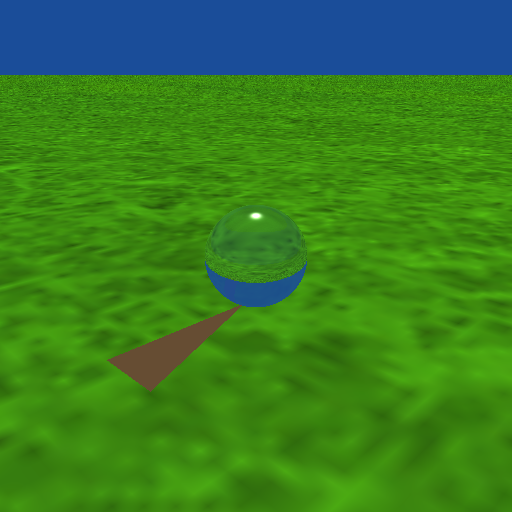
\includegraphics[width =\textwidth]{./Worksheet3/MagnifRenduInterpo.png}\\
				\textit{Linear sampling (interpolation) with a scaling factor divided by 10 (0.02 instead of 0.2)}
			\end{center}
		\end{minipage}
	\end{center}
	
	With the nearest sampling we can clearly distinguish the same texels covering multiple pixels, this implies big squares of the same color and a big discontinuity in between. This problem is diminished with the interpolation implementation as pixel values are interpolated between texel values, thus the resulting image is smoothed.
	
	%%%%%%%%%%%%%%%%%%%%%%%%%%%%%%%%%%%%%%%%%%%%%%%%%%%%%%%%
	% 						                  	PART 4
	%%%%%%%%%%%%%%%%%%%%%%%%%%%%%%%%%%%%%%%%%%%%%%%%%%%%%%%%
	\section{Worksheet 4}
	\subsection{Cornell box and blocks}
	Loading the Cornell box and blocks using the command line \textit{./raytraced ../models/CornellBox.obj ../models/CornellBlocks.obj} leads to the following base colour preview:
	\begin{center}
		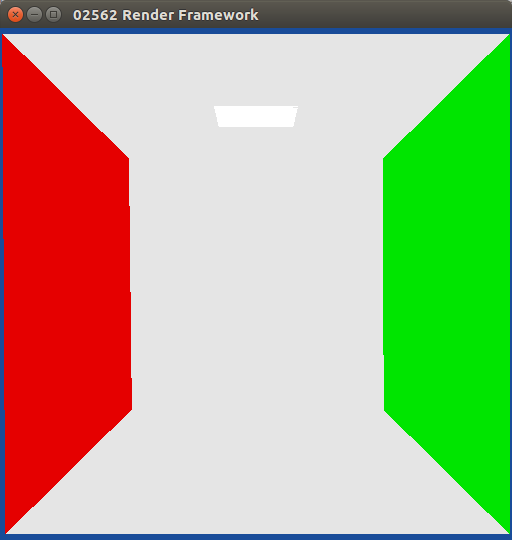
\includegraphics[width=8cm]{./Worksheet4/CornellBasePreview}\\
		\textit{Cornell box and blocks preview}
	\end{center}
	
	After implementing the \textit{intersect} function in \textbf{TriMesh.cpp} the render result is the same as preview:
	\begin{lstlisting}
	bool TriMesh::intersect(const Ray& r, HitInfo& hit, unsigned int prim_idx) const
	{
		const uint3& face = geometry.face(prim_idx);
		
		float3 v0 = geometry.vertex(face.x);
		float3 v1 = geometry.vertex(face.y);
		float3 v2 = geometry.vertex(face.z);
		float3 normal;
		float dist, v ,w;

		bool intersects = ::intersect_triangle(r, v0, v1, v2, normal, dist, v, w);
		
		if (intersects) {
			hit.has_hit = true;
			hit.dist = dist;
			hit.geometric_normal = normalize(normal);
			// Set the shading normal to geometric normal for now
			hit.shading_normal = hit.geometric_normal;
			
			hit.position = r.origin + r.direction*dist;
			hit.material = &(materials[mat_idx[prim_idx]]);
		}
		return intersects;
	}
	\end{lstlisting}
	
	\begin{center}
		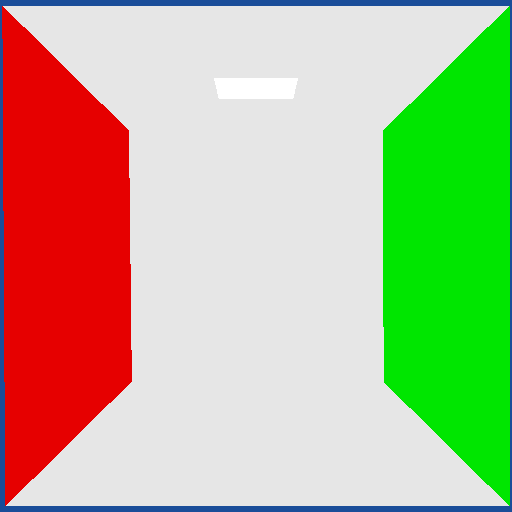
\includegraphics[width=8cm]{./Worksheet4/cornellblocks_flat.png}\\
		\textit{Cornell box and blocks rendering with default directional light}
	\end{center}
	
	To display the Cornell scene we implement the area light in \textbf{AreaLight.cpp}:
	
	\begin{lstlisting}
	bool AreaLight::sample(const float3& pos, float3& dir, float3& L) const
	{
		const IndexedFaceSet& normals = mesh->normals;
		L = make_float3(0.0f);
		
		float3 center = mesh->compute_bbox().center();
		dir = center - pos;
		float dist = length(dir);
		dir = normalize(dir);
		
		// Test if in shadows with shadow ray
		Ray shadow_ray = Ray(center, -dir, 0, 1e-4, dist - 1e-4);
		HitInfo hit;
		if (shadows & tracer->trace_to_any(shadow_ray, hit)) {
			// return false with L still equal to zero
			return false;
		}
		
		// Not in shadows
		// For each triangle in the mesh
		for (int i = 0; i < mesh->normals.no_faces(); i++) {
			uint3 face = normals.face(i);
			float3 normal_mean = normalize(normals.vertex(face.x) + normals.vertex(face.y) + normals.vertex(face.z));
			double dotProduct = -dot(dir, normal_mean);
			dotProduct = fmax(dotProduct, 0);
			L += make_float3(dotProduct * mesh->face_areas[i]) * get_emission(i);
		}
		
		// Fr and dot product handled by Lambertian
		L /= pow(dist, 2);
		
		return true;
	}
	\end{lstlisting}
	
	
	Then we can compare the preview with rendered scene:
	\begin{center}
		\begin{minipage}[b]{0.40\linewidth}
			\begin{center}
				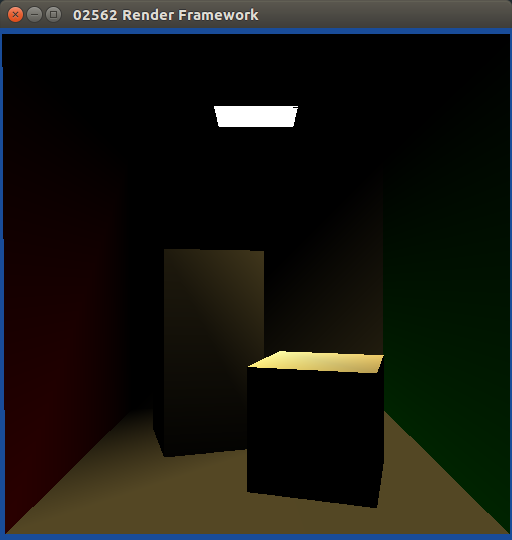
\includegraphics[width = \textwidth]{./Worksheet4/preview_cornell_area.png}\\
				\textit{Preview of the Cornell scene with area light}
			\end{center}
		\end{minipage}
		\hspace{0.05\linewidth}
		\begin{minipage}[b]{0.40\linewidth}
			\begin{center}
				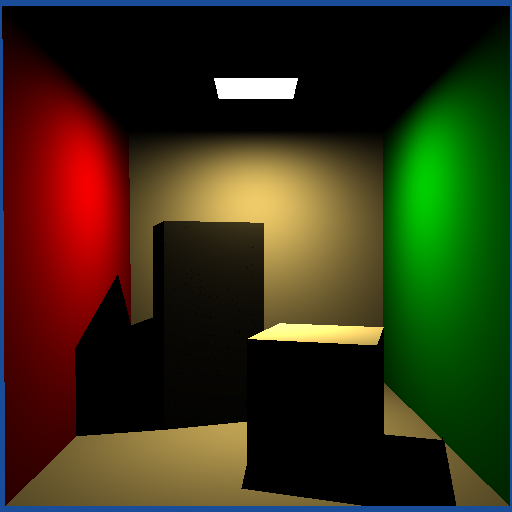
\includegraphics[width =\textwidth]{./Worksheet4/cornellblocks_render.png}\\
				\textit{Rendering of the Cornell scene with area light}
			\end{center}
		\end{minipage}
	\end{center}
	
	For the Utah teapot, the \textit{Directional Light} is needed:
	\textbf{Directional.cpp}
	
	\begin{lstlisting}
	bool Directional::sample(const float3& pos, float3& dir, float3& L) const
	{
		dir = -light_dir;
		L = make_float3(0.0f);
		
		Ray shadowRay(pos, dir, 0, 1e-4, 10.0f);
		HitInfo hit;
		if (shadows & tracer->trace_to_any(shadowRay, hit)){
			// return with L = 0.0f
			return false;
		}
		
		// Fr and dot product handled by Lambertian
		L = emission;
		
		return true;
	}
	\end{lstlisting}
	
	We then can render the teapot, as the mesh is big and we don't have space subdivision the rendering is longer and takes approximately 300s. We can see that the rendering is not smooth and we can see each square composing the mesh, to make it smooth we can compute the normals along the faces using the barycentric coordinates in \textbf{TriMesh.cpp}:
	
	\begin{lstlisting}
	bool TriMesh::intersect(const Ray& r, HitInfo& hit, unsigned int prim_idx) const
	{
		const uint3& face = geometry.face(prim_idx);
		
		float3 v0 = geometry.vertex(face.x);
		float3 v1 = geometry.vertex(face.y);
		float3 v2 = geometry.vertex(face.z);
		float3 normal;
		float dist, v ,w;
		
		bool intersects = ::intersect_triangle(r, v0, v1, v2, normal, dist, v, w);
		
		if (intersects) {
			hit.has_hit = true;
			hit.dist = dist;
			hit.geometric_normal = normalize(normal);
			
			if (has_normals()) {
				uint3 normals_idx = normals.face(prim_idx);
				float3 n1 = normals.vertex(normals_idx.x);
				float3 n2 = normals.vertex(normals_idx.y);
				float3 n3 = normals.vertex(normals_idx.z);
				float3 interp_normal = normalize((1-v-w)*n1 + v*n2 + w*n3);
				hit.shading_normal = interp_normal;
			} else {
				hit.shading_normal = hit.geometric_normal;
			}
			
			hit.position = r.origin + r.direction*dist;
			hit.material = &(materials[mat_idx[prim_idx]]);
		}
		return intersects;
	}
	\end{lstlisting}
	
	We obtain the following renderings:
	\begin{center}
		\begin{minipage}[b]{0.40\linewidth}
			\begin{center}
				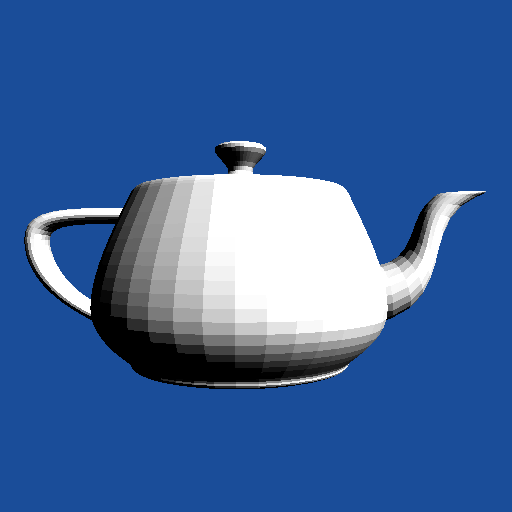
\includegraphics[width = \textwidth]{./Worksheet4/teapot_raw.png}\\
				\textit{Teapot rendering using face normals
					\vspace{2.2em}}\\
			\end{center}
		\end{minipage}
		\hspace{0.05\linewidth}
		\begin{minipage}[b]{0.40\linewidth}
			\begin{center}
				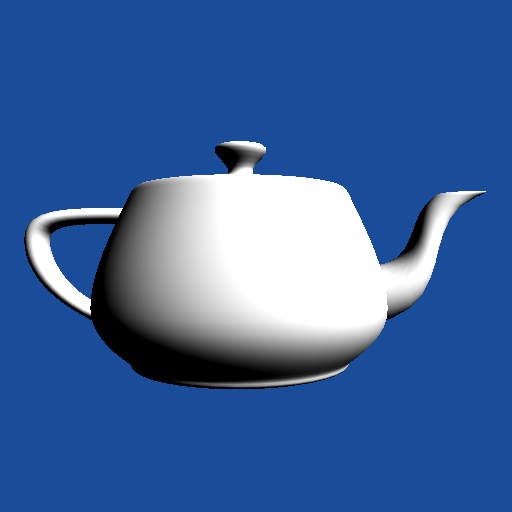
\includegraphics[width =\textwidth]{./Worksheet4/teapot_smooth.png}\\
				\textit{Teapot rendering using normals barycentric interpolation across triangles}
			\end{center}
		\end{minipage}
	\end{center}
	
	\subsection{BSP Tree}
	The naive intersection method consists in testing intersection with all rays, this is very costly, especially if the number of triangles in the mesh is very high. A lot of intersection tests are made with triangles which are far away from our ray.\\
	
	In order to improve this intersection algorithm we use a recursive intersection method involving a \textit{BSP tree}. This BSP tree is first constructed iteratively with the object bounding box as the root and then subdivide this bounding box along an axis-aligned plane, to create two children with smaller (and adjusted to smaller parts of the object) bounding boxes. When we reach a certain criteria (size of bounding boxes, number of primitives inside a leaf bounding box..) we stop the tree growth.\\
	
	A hard point is to find the best subdivision plane in order to chose the more efficient subdivision regarding the size of the produced children bounding boxes and the primitives inside each. To optimize it without being too costly, we compute some different subdivisions and choose the one with the minimal cost($= \sum number\_of\_primitives\_inside\_bounding\_box*size\_of\_bounding\_box$).\\
	
	Once this structure is constructed, testing intersection is then an easy recursive search. Starting from the root, if the ray intersect the bounding\_box of the considered node (\textit{intersect\_node} function), we test if it intersects its children, if it intersects one then we recursively call the \textit{interest\_node} on this node and so on. When we reach a tree leaf, we just have to test the intersection as we did before with the primitives in this leaf. Due to tree construction the number of primitives in each leaf should be really low and then we only compute a small number of ray-primitive intersections regarding the old naive method without altering the rendered result.\\
	
	To use this structure in our program we have to modify the \textit{closest\_hit} and \textit{any\_hit} functions in the file \textbf{BspTree.cpp}:\\
	
	\begin{lstlisting}
	bool BspTree::closest_hit(Ray& r, HitInfo& hit) const
	{
		closest_plane(r, hit);
		// Test with biggest bounding box first
		if (intersect_min_max(r)) {
			// Start at the root
			BspNode root = *this->root;
			intersect_node(r, hit, root);
		}
		return hit.has_hit;
	}
	\end{lstlisting}
	
	\begin{lstlisting}
	bool BspTree::any_hit(Ray& r, HitInfo& hit) const
	{
		if (any_plane(r, hit)){
			return true;
		}
		    
		// Test if it intersects the biggest bounding box first
		if (!intersect_min_max(r)) {
			return false;
		}
		// Start at the root
		BspNode root = *this->root;
		return intersect_node(r, hit, root);
	}
	\end{lstlisting}
	
	To compare the renderings time and measure the speedup, the time of rendering was recorded 5 times and then averaged, this for the differentgeometries (except the Stanford Rabbit whose rendering time for the Naive Algorithm was too long):\\
	
	\begin{tabular}{|l|c|c|c|}
		\hline
		\textbf{Time (s)} & \textbf{Cornell Boxes} & \textbf{Teapot} & \textbf{Stanford Rabbit}\\ \hline \hline
		Naive (Without BSP) & 2.553 & 236.77 &57m38s\\ \hline
		& 2.587 & 232.01 &/\\ \hline
		& 2.597 & 232.69 &/\\ \hline
		& 2.537 & 293.93 &/\\ \hline
		& 2.617 & 229.48 &/\\ \hline
		\textit{Mean} & 2.578 & 244.98 &57m38s\\ \hline \hline
		With BSP & 1.098 & 0.4903 & 1.554\\ \hline
		& 1.064 & 0.5245 & 1.465\\ \hline
		& 1.073 & 0.4903 & 1.454\\ \hline
		& 1.086 & 0.4900 & 1.485\\ \hline
		& 1.069 & 0.4878 & 1.454\\ \hline
		\textit{Mean} & 1.078 & 0.4966 & 1.482\\ \hline \hline
		\textbf{Speedup} & 2.40 & 493.3 &2333\\ \hline
	\end{tabular}
	\vspace{1em}
	
	Where $Speedup = \frac{Mean_{Naive}}{Mean_{BSP}}$.\\
	
	
	We can clearly see the time speedup between the BSP-tree algorithm and the naive way. On reasonable geometries such as the \textit{Teapot}, the rendering time is almost divide by 500. On smaller geometries (\textit{Cornell Boxes}) the gain is obviously smaller as fewer triangles are present in the meshes. For the stanford rabbit, which contains near to 70\ 000 triangles, the rendering time using the naive intersection algorithm is astronomic and we can achieve a speedup of about 2300.
	

	%%%%%%%%%%%%%%%%%%%%%%%%%%%%%%%%%%%%%%%%%%%%%%%%%%%%%%%%
	% 						                  	PART 5
	%%%%%%%%%%%%%%%%%%%%%%%%%%%%%%%%%%%%%%%%%%%%%%%%%%%%%%%%
	\section{Worksheet 5}
	
	\subsection{Part 1}
	We have the following informations:
	$$
	\begin{cases}
		P = 25W\\
		\rho = 20\%\\
		\lambda = 500nm
	\end{cases}
	$$
	
	As the light bulb has an efficiency of $\rho = 20\%$, the power emitted by this bulb is :
	\begin{align*}
	P_e &= \rho P\\
	&= 0.2*25\\
	&= 5W
	\end{align*}
	
	We know the wavelength $\lambda$ emitted by this lamp, thus:
	$$
	f = \frac{c}{\lambda} = \frac{3*10^{8}}{500*10^{-9}} = 6*10^{14} s^{-1}$$
	$$
	q[500nm] = hf = 6.63*10^{-34} * 6*10^{14} s^{-1} \approx 4*10^{-19}
	$$
	
	The, we can compute the approximate number of photons emitted per second :
	$$
	N_{photon}[5W] = \frac{5}{4*10^{-19}} = \boxed{1.25*10^{18}\ photons/s}
	$$
	
	\subsection{Part 2}
	We have :
	$$
	\begin{cases}
		U = 2.4V\\
		I = 0.7A\\
		d = 1cm = 10^{-2}m
	\end{cases}
	$$
	The \textit{Radiant Flux} correspond to the emitted power:
	$$
	\Phi = P = UI = 2.4*0.7 = \boxed{1.68W}
	$$
	
	As the light bulb is approximatively sphere-shaped and emits light equally in all directions (isotropic) we have, for the \textit{Radiant Intensity}:
	$$
	I = \frac{\Phi}{4\pi} = \frac{1.68}{4*\pi} \approx \boxed{1.34*10^{-1} W/sr}
	$$
	We can then deduce the \textit{Radiant Exitance}:
	$$
	M = \frac{\Phi}{4\pi r^2} = \frac{1.68}{4*\pi*(\frac{10^{-2}}{2})^2} = \boxed{5.35*10^3 W/m^2}
	$$
	Finally, as $\Phi = \frac{dQ}{dt}$, we have for the \textit{Emitted Energy} during 5min:
	$$
	Q = \int_T \Phi dt = \Phi t = 1.68*5*60 = \boxed{504J}
	$$
	 
	\subsection{Part 3}
	Let $R = 1m$ the distance between the light bulb and the eye, $r = 3mm$ (as the pupil diameter is 6mm) the pupil opening.
	
	From the preceding exercise we know that, for this light bulb:
	$$
	I = 1.34*10^{-1} W/sr
	$$
	Then, we can compute the irradiance received by the eye with the formula:
	$$
	E = I\frac{\cos(\theta)}{r^2}
	$$
	As the eye is very small considered the distance to the light bulb, and looking directly at the light we have $\theta = 0$, then:
	$$
	E = I\frac{\cos(0)}{1^2} = \boxed{I = 1.34*10^{-1} W/m^2}
	$$
	
%At this distance from the light, and as the pupil is very small, we can approximate its area as a disc area. As we have, for the solid angle $\Omega = \frac{A}{R^2}$ where A is the pupil area, then:
%	$$
%	\Omega = \frac{4\pi r^2}{R^2} = \frac{\pi*(3*10^{-3})^2}{1^2} \approx \boxed{2.83*10^{-5}}
%	$$
%	
%	We have then:
%	$$
%	\Phi = \int_{\Omega} E.dA = E \int_{\Omega_{pupil}} dA = E.A_{pupil}
%	$$
%	And $\Phi = 1.68W$ from the preceding exercise, thus:
%	$$
%	E = \frac{\Phi}{A_{pupil}}= \frac{\Phi}{\pi r^2} = \frac{1.68}{\pi * (3*10^{-3})^2} = \boxed{5.94*10^4 W/m^2}
%	$$
	
%	, and $\theta$ the angle as defined below:
%	\begin{center}
%		\includegraphics[width=10cm]{./Worksheet5/IMAG1865.jpg}
%	\end{center}
%	
%	We thus have:
%	$$
%	\tan(\theta) = \frac{r}{d} = \frac{3*10^{-3}}{1} = 3*10^{-3}
%	$$
%	$$
%	\theta = \arctan(3*10^{-3}) \approx 3*10^{-3} radian
%	$$
	
	
	
	\subsection{Part 4}
	From the problem, we have:
	$$
	\begin{cases}
	P_u = 200W\\
	\rho = 20\%\\
	d = 2m\\
	\lambda = 650nm
	\end{cases}
	$$	
	
	To calculate the \textit{Irradiance} at the point of the table right under the light (thus $\theta = 0$) bulb we use the same formula as in the precedent exercise:
	\begin{align*}
		E &= I\frac{cos(\theta)}{d^2}\\
		&= I\frac{cos(0)}{d^2}\\
		&= \frac{\Phi}{4\pi}\frac{1}{d^2}\\
		&= \frac{P\rho}{4\pi}\frac{1}{d^2}\\
		&= \frac{200*0.2}{4*\pi}\frac{1}{2^2}\\
		&= \boxed{0.796\ W/m^2}
	\end{align*}
	
	
	As we have the following relation between photometric and radiometric measurements:
	$$
	Photometric = Radiometric * 685 * V(\lambda)
	$$
	Where $V(\lambda)$ is the luminous efficiency curve, with $V(650nm) = 0.1$. Using the \textit{Irradiance E} antecedently found we have:
	$$
	Illuminance = E * 685 * V(\lambda) = E*685*V(650) \approx 0.796*685*0.1 \approx \boxed{54.51\ Lux}
	$$
	
	\subsection{Part 5}
	Let $r_x$ (and respectively $r_s$) be the distance from the known source (resp the unknown) and the screen. At the matching position, bot light sources have the same irradiance on the screen (measured by a photometer). We know that the \textit{Radiant Flux} is defined by:
	$$
	\Phi = E \int_{\Omega}dA = E*4*\pi*r^2 \text{ (For a sphere with a radius } r \text{)}
	$$
	And:
	$$
	\Phi = 4*\pi*I
	$$
	
	We thus have:
	$$
	E = \frac{\Phi}{4\pi r^2} = \frac{4\pi I}{4\pi r^2} = \frac{I}{r^2}
	$$
	
	At the screen position defined by $r_x$ and $r_s$ we have $K(\lambda)E_x = K(\lambda)E_s$ as we use a photometer (sensibility to different wavelength), thus:
	\begin{align*}
	&\frac{I_s K(\lambda)}{r_s^2} = \frac{I_x K(\lambda)}{r_x^2}\\
	&\iff \frac{I_s}{r_s^2} = \frac{I_x}{r_x^2}\\
	&\iff I_x = I_s \frac{r_x^2}{r_s^2}\\
	&\iff I_x = 40*\frac{65*10^{-2}}{35*10^{-2}} \approx \boxed{138\ cd}
	\end{align*}
	
	\subsection{Part 6}
%	$$
%	M = \frac{d\Phi}{dA}
%	$$
%	$$
%	L = \frac{d\Phi}{dA^\perp d\omega}
%	$$
	As we are considering a diffuse emitter, we know that:
	$$
	\Phi = LA\pi
	$$
	As $E = \frac{\Phi}{A}$, we have:
	$$
	E = \frac{LA\pi}{A} = L\pi = 5000*\pi \approx \boxed{15708\ W/m^2}
	$$
	
	As $E = \frac{d\Phi}{dA}$, we can find the emitted energy using the area of this light:
	$$
	\Phi = E*A \approx 15708*0.1*0.1 \approx \boxed{157.08\ W}
	$$
	
	\subsection{Part 7}
	We have the following formulas for \textit{Radiant Excitance M} and \textit{Radiance L}:
	$$
	M = \frac{d\Phi}{dA}
	$$
	$$
	L = \frac{d\Phi}{dA^\perp d\omega} = \frac{d\Phi}{dA \cos(\theta)d\omega}
	$$
	We thus have :
	\begin{align*}
		M &= \int_{2\pi} L\cos(\theta)d\omega\\
		&= \int_{\phi = 0}^{2\pi}\int_{\theta = 0}^{\pi/2} L \cos(\theta) \sin(\theta) d\theta d\phi\\
		&= \int_{\phi = 0}^{2\pi}\int_{\theta = 0}^{\pi/2} 6000 \cos^2(\theta) \sin(\theta) d\theta d\phi\\
		&= 6000\left(\int_{\phi = 0}^{2\pi} d\phi\right)\left(\int_{\theta = 0}^{\pi/2}\cos^2(\theta) \sin(\theta) d\theta\right)\\
		&= 6000*2\pi*\left[-\frac{\cos^3(\theta)}{3}\right]_{0}^{\pi/2} \quad \hspace{2em}\quad \textit{Because } \frac{d\cos(\theta)}{d\theta} = -\sin(\theta)\\
		&= 6000*2\pi*[0 - \frac{-1}{3}]\\
		&= 6000*2\pi*\frac{1}{3}\\
		&\approx \boxed{12566\ W/m^2}
	\end{align*}
	
	From this we can deduce the emitted power as in the precedent exercise:
	$$
	\Phi = M * A \approx 12566*0.1*0.1 \approx \boxed{125.66\ W}
	$$
	
	%%%%%%%%%%%%%%%%%%%%%%%%%%%%%%%%%%%%%%%%%%%%%%%%%%%%%%%%
	% 						                  	PART 6
	%%%%%%%%%%%%%%%%%%%%%%%%%%%%%%%%%%%%%%%%%%%%%%%%%%%%%%%%
	\section{Worksheet 6}
	The pixel subdivision level can be changed using the keys '+' and '-' to respectively increase and decrease the number of jitter samples per pixel in a simple ray tracing. Any modification imply a re-computation of the jitters using the function \textit{compute\_jitters}.
	
	This function stores in the \textit{jitter} array, for each subdivision of this pixel, the displacement from the pixel center to the randomly sub-pixel jitter computed. When the pixel subdivision level is set to $s$ we get $s^2$ sub-pixels for each pixel, as we subdivide our pixel using $s$ portions in each dimension (height, width).
	
	Casting a reay through each sub-pixel and averaging their values is done in the \textit{compute\_pixel} function in \textbf{RayCaster.cpp}:
	
	\begin{lstlisting}
	float3 RayCaster::compute_pixel(unsigned int x, unsigned int y) const
	{
		int n_subpixels = pow(subdivs, 2);
		float3 result = make_float3(0.0f);
		float xip = x * win_to_ip.x + lower_left.x;
		float yip = y * win_to_ip.y + lower_left.y;
		
		for (int i = 0; i < n_subpixels; i++) {
			float2 displacement = jitter[i];
			float2 coords = make_float2(xip + displacement.x, yip + displacement.y);
			
			Ray r = scene->get_camera()->get_ray(coords);
			
			HitInfo hit = HitInfo();
			scene->closest_hit(r, hit);
			
			if (hit.has_hit) {
				result += get_shader(hit)->shade(r, hit);
				} else {
				result += get_background();
			}
		}
		return result/n_subpixels;
	}
	\end{lstlisting}
	
	Increasing the subdivision level $s$ leads to significant improvement in reduction of aliasing effect (the stairing effect on sharp edges become less visible as we increase $s$) but increase also proportionally the rendering time:
	
	\begin{center}
	\begin{tabular}{|c|c|}
		\hline
		Subdivision level $s$ & Rendering time (s) (averaged on 3 realizations)\\ \hline
		1 & 1.02\\ \hline
		2 & 3.98\\ \hline
		3 & 9.04\\ \hline
		4 & 16.25\\ \hline
		5 & 25.57\\ \hline
		6 & 36.27\\ \hline
	\end{tabular}
	\end{center}
	
	From these results, we can see that the rendering time is proportional to the subdivision level squared ($R_{time} \propto s^2$). Indeed, for each pixel the ray-tracing is done $s^2$ times, this part being the more costly in rendering we increase the rendering time proportionally to the number of repetitions.
	
	TODO : MATHEMATICAL describe the (worst case) mathematical relationship between subdivision level and aliasing error\\
	
	For the original rendering image size, a pixel subdivision level of $s = 3$ gives already good results, without driving the rendering time too high. A pixel subdivision level greater than $s = 4$ is too costly regarding the increase of rendering time it involves. Below is the different renders for the Cornell box and blocks with stratified sampling for $s$ from 1 to 6:
	
	
	\begin{center}
		\begin{minipage}[b]{0.40\linewidth}
			\begin{center}
				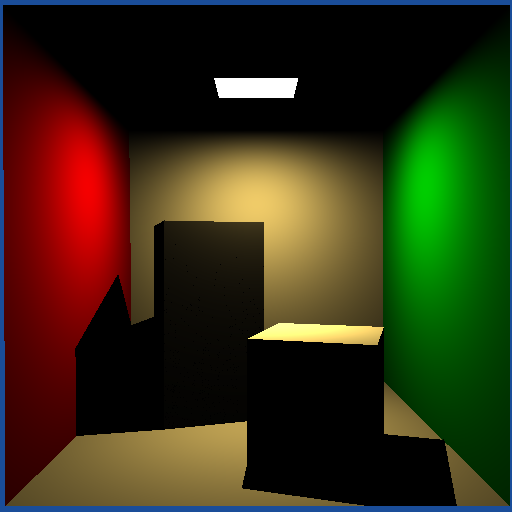
\includegraphics[width = \textwidth]{./Worksheet6/cornellblocks1.png}\\
				\textit{s = 1}
			\end{center}
		\end{minipage}
		\hspace{0.05\linewidth}
		\begin{minipage}[b]{0.40\linewidth}
			\begin{center}
				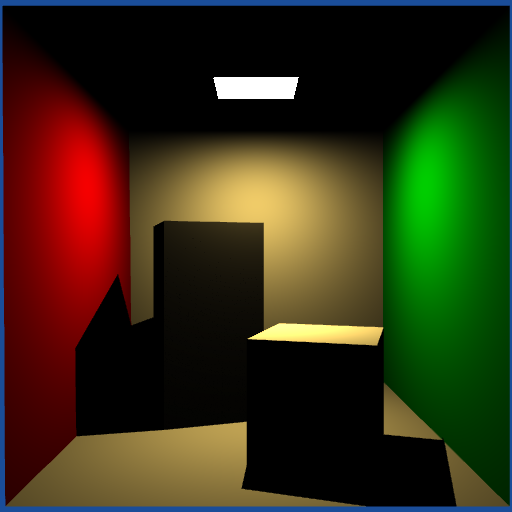
\includegraphics[width = \textwidth]{./Worksheet6/cornellblocks2.png}\\
				\textit{s = 2}
			\end{center}
		\end{minipage}
	\end{center}
	
	\begin{center}
		\begin{minipage}[b]{0.40\linewidth}
			\begin{center}
				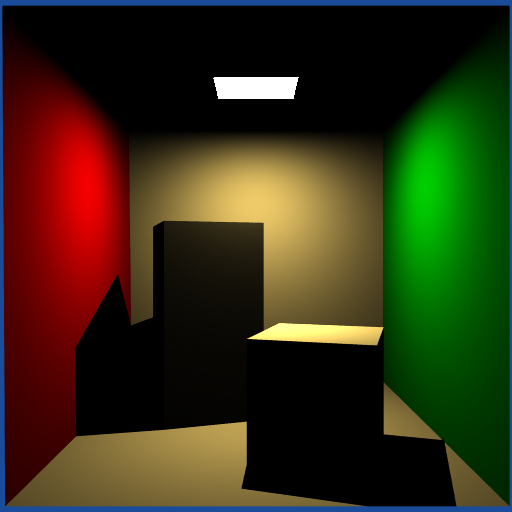
\includegraphics[width = \textwidth]{./Worksheet6/cornellblocks3.png}\\
				\textit{s = 3}
			\end{center}
		\end{minipage}
		\hspace{0.05\linewidth}
		\begin{minipage}[b]{0.40\linewidth}
			\begin{center}
				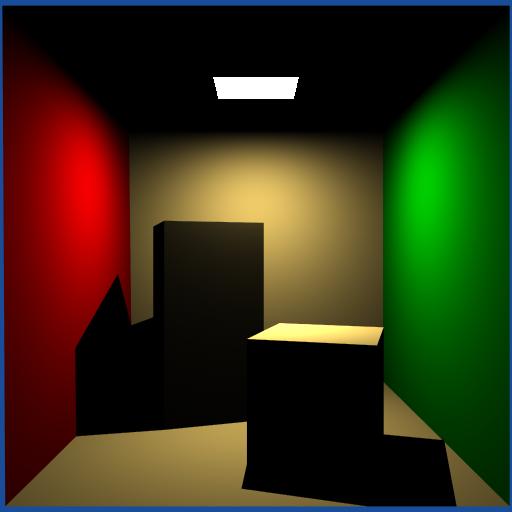
\includegraphics[width = \textwidth]{./Worksheet6/cornellblocks4.png}\\
				\textit{s = 4}
			\end{center}
		\end{minipage}
	\end{center}
	
	\begin{center}
		\begin{minipage}[b]{0.40\linewidth}
			\begin{center}
				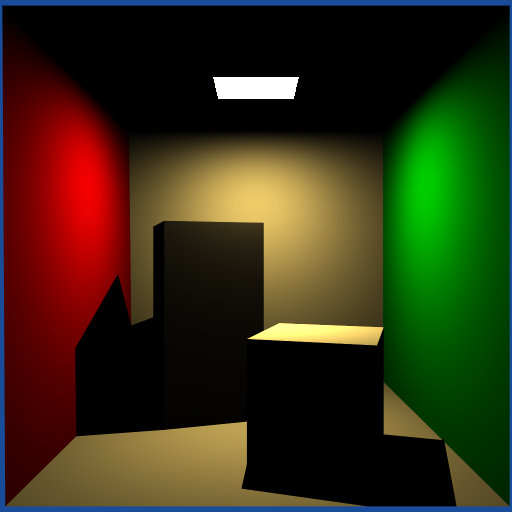
\includegraphics[width = \textwidth]{./Worksheet6/cornellblocks5.png}\\
				\textit{s = 5}
			\end{center}
		\end{minipage}
		\hspace{0.05\linewidth}
		\begin{minipage}[b]{0.40\linewidth}
			\begin{center}
				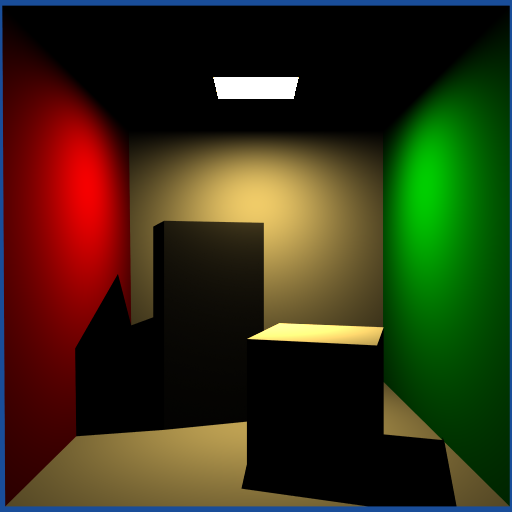
\includegraphics[width = \textwidth]{./Worksheet6/cornellblocks6.png}\\
				\textit{s = 6}
			\end{center}
		\end{minipage}
	\end{center}
	
	\section{Worksheet 7}
	Emitting photons from the point light is implemented in \textbf{PointLight.cpp}:
	
	\begin{lstlisting}
	bool PointLight::emit(Ray& r, HitInfo& hit, float3& Phi) const
	{		
		// Sample ray direction and create ray
		float x, y, z;
		do {
			x = mt_random() * 2 - 1; // Random value between -1 and 1
			y = mt_random() * 2 - 1; // Random value between -1 and 1
			z = mt_random() * 2 - 1; // Random value between -1 and 1
		} while (pow(x, 2) + pow(y, 2) + pow(z, 2) > 1);
		float3 dir = make_float3(x, y, z);
		
		// Trace ray
		r = Ray(light_pos, dir, 0, 1e-4, RT_DEFAULT_MAX);
		
		// If a surface was hit, compute Phi and return true
		if (tracer->trace_to_any(r, hit)) {
			//Surface was hit
			Phi = intensity*4*M_PIf;
			return true;
		}
		
		return false;
	}
	\end{lstlisting}
	
	We can then trace these photons to the first diffuse surface, considering a maximum amount of reflections/refractions to reach this surface. The photons which have been reflected or refracted at least once and then reached this surface are then stored in a \textit{caustic photon map}. This process is done in \textbf{ParticleTracer.cpp}:
	\begin{lstlisting}
	void ParticleTracer::trace_particle(const Light* light, const unsigned int caustics_done)
	{
		if(caustics_done)
		return;
		
		// Shoot a particle from the sampled source
		Ray r;
		HitInfo hit;
		float3 Phi;
		if (!light->emit(r, hit, Phi)) {
			// If no hit at all
			return;
		}
		
		// Forward from all specular surfaces
		while(scene->is_specular(hit.material) && hit.trace_depth < 500)
		{
			switch(hit.material->illum)
			{
				case 3:  // mirror materials
				{
					// Forward from mirror surfaces
					Ray r_out;
					HitInfo hit_out;
					if (!trace_reflected(r, hit, r_out, hit_out)) {
						return;
					}
					r = r_out;
					hit = hit_out;
				}
				break;
				case 11: // absorbing volume
				case 12: // absorbing glossy volume
				{
					// Handle absorption here (Worksheet 8)
				}
				case 2:  // glossy materials
				case 4:  // transparent materials
				{
					// Forward from transparent surfaces
					Ray r_out;
					HitInfo hit_out;
					
					// Russian roulette to choose between reflection and refraction
					float P;
					trace_refracted(r, hit, r_out, hit_out, P);
					if (mt_random() < P) {
						hit_out.has_hit = false;
						trace_reflected(r, hit, r_out, hit_out);
					}
					
					if (!hit_out.has_hit) {
						return;
					}
					
					r = r_out;
					hit = hit_out;
				}
				break;
				default:
				return;
			}
		}
		
		// Store in caustics map at first diffuse surface
		if (hit.trace_depth > 0)
		caustics.store(Phi, hit.position, -r.direction);
	}
	\end{lstlisting}
	The render parameters are set as :
	\begin{itemize}
		\item Number of photons in map = 100 000
		\item Number of photons in the radiance estimate for caustics = 200 000
		\item Number of jitter samples = 1 per pixel
	\end{itemize}
	We obtain the following photon distribution in the default scene:
	
	\begin{center}
		\begin{minipage}[b]{0.40\linewidth}
			\begin{center}
				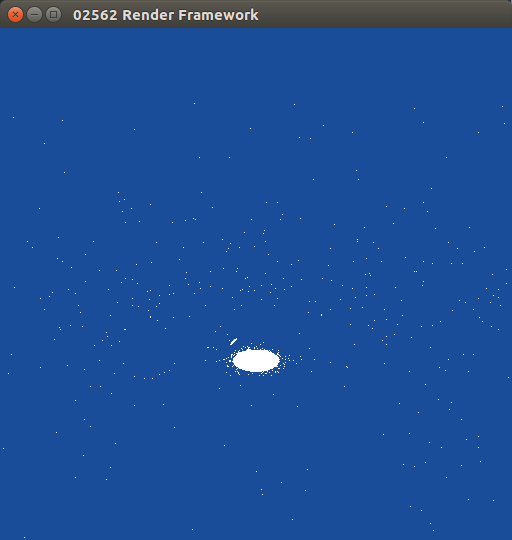
\includegraphics[width = \textwidth]{./Worksheet7/causticphotons.png}\\
				\textit{Photo distribution in default scene}
			\end{center}
		\end{minipage}
	\end{center}
	
	Writing the associated shader allows to visualize the caustic effects, alone and superposed with other Lambertian illumination. As the shader returns a \textit{radiance} value and we \textit{caustic photon map} stores irradiance we have to transform it:
	$$
	\text{Irradiance : } E = \frac{d\Phi}{dA}
	$$
	$$
	\text{Reflected light : } L_r = \int_{2*\pi} f_r L_i \cos{\theta} d\omega
	$$
	As we are considering diffuse materials, their BRDF is : $ f_r = \frac{\rho_d}{\pi}$, and as the irradiance estimate is $dE = L_i \cos{\theta} d\omega$ we have :
	\begin{align*}
	\hspace{10em} L_r &= \int_{2\pi} f_r dE\\
	&\approx \frac{1}{n_{photons}} \sum_{photons} f_r \frac{\Delta \Phi_p}{\Delta_A}\\
	&= f_r \frac{1}{n_{photons}} \sum_{photons} \frac{\Delta \Phi_p}{\Delta_A} \hspace{2em} \text{as the material is diffuse}
	\end{align*}
	\textbf{PhotonCaustics.cpp}
	
	\begin{lstlisting}
	float3 PhotonCaustics::shade(const Ray& r, HitInfo& hit, bool emit) const
	{
		float3 brdf = rho_d*M_1_PIf;
		float3 irradiance = tracer->caustics_irradiance(hit, max_dist, photons);
		
		return brdf*irradiance + Lambertian::shade(r, hit, emit);
	}
	\end{lstlisting}
	
	This leads to the following renderings on the default scene:
	
	\begin{center}
		\begin{minipage}[b]{0.40\linewidth}
			\begin{center}
				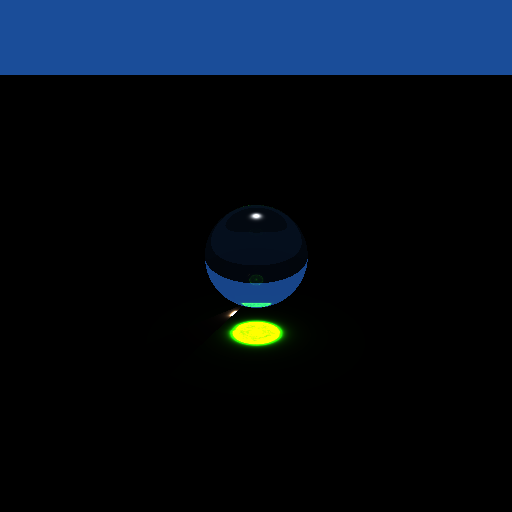
\includegraphics[width = \textwidth]{./Worksheet7/causticsrender.png}\\
				\textit{Rendering with caustics only}\\
				\vspace{1em}
			\end{center}
		\end{minipage}
		\hspace{0.05\linewidth}
		\begin{minipage}[b]{0.40\linewidth}
			\begin{center}
				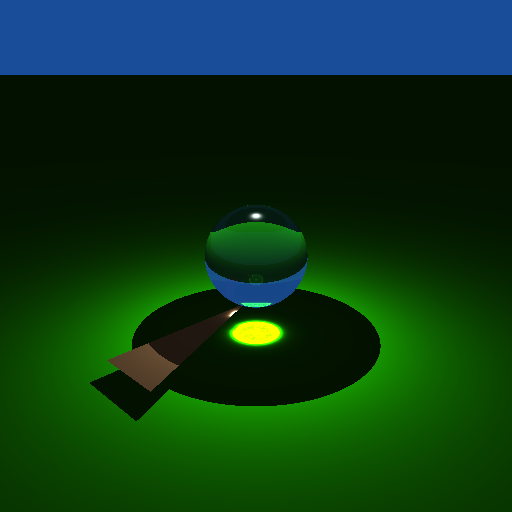
\includegraphics[width = \textwidth]{./Worksheet7/causticsandillumination.png}\\
				\textit{Rendering with caustics and other illumination}
			\end{center}
		\end{minipage}
	\end{center}
	
	\section{Worksheet 8}
	\subsection{Fresnel reflectance}
	After implementing the fresnel reflectance in \textbf{fresnel.h} allows the variation of the reflectance coefficient around the ball according to the angle of view and refractive indices:
	\begin{lstlisting}
	inline float fresnel_r_s(float cos_theta1, float cos_theta2, float ior1, float ior2)
	{
		// Compute the perpendicularly polarized component of the Fresnel reflectance
		return (ior1*cos_theta1 - ior2*cos_theta2)/(ior1*cos_theta1 + ior2*cos_theta2);
	}
	
	inline float fresnel_r_p(float cos_theta1, float cos_theta2, float ior1, float ior2)
	{
		// Compute the parallelly polarized component of the Fresnel reflectance
		return (ior2*cos_theta1 - ior1*cos_theta2)/(ior2*cos_theta1 + ior1*cos_theta2);
	}
	
	inline float fresnel_R(float cos_theta1, float cos_theta2, float ior1, float ior2)
	{
		// Compute the Fresnel reflectance using fresnel_r_s(...) and fresnel_r_p(...)
		return (pow(fresnel_r_s(cos_theta1, cos_theta2, ior1, ior2), 2) + pow(fresnel_r_p(cos_theta1, cos_theta2, ior1, ior2), 2))/2;
	}
	\end{lstlisting}
	
	In \textbf{RayTracer.cpp} we have to be careful when computing the $R$ coefficient, indeed the incident ray direction is toward the surface (in the opposite direction of the surface normal) and the refracted ray direction must be compared with the inversed normal (normal inside the material):
	\begin{lstlisting}
		bool RayTracer::trace_refracted(const Ray& in, const HitInfo& in_hit, Ray& out, HitInfo& out_hit, float& R) const
		{
			float3 normal;
			float cos_theta_in;
			out_hit.ray_ior = get_ior_out(in, in_hit, out.direction, normal, cos_theta_in);
			out_hit.trace_depth = in_hit.trace_depth + 1;
			
			bool is_refracted = optix::refract(out.direction, in.direction, normal, out_hit.ray_ior/in_hit.ray_ior);
			if (!is_refracted) {
				// Detect total internal reflection
				R = 1;
				return false;
			}
			
			R = fresnel_R(dot(normal, -in.direction), dot(-normal, out.direction), in_hit.ray_ior, out_hit.ray_ior);
			out.origin = in_hit.position;
			out.ray_type = 0;
			out.tmax = RT_DEFAULT_MAX;
			out.tmin = 1.0e-4f;
			
			return trace_to_closest(out, out_hit);
		}
	\end{lstlisting}
	
	We can then compare the \textit{Transparent} shader depending if the reflectance $R$ is kept constant or computed using fresnel equations:
	
	\begin{center}
		\begin{minipage}[b]{0.40\linewidth}
			\begin{center}
				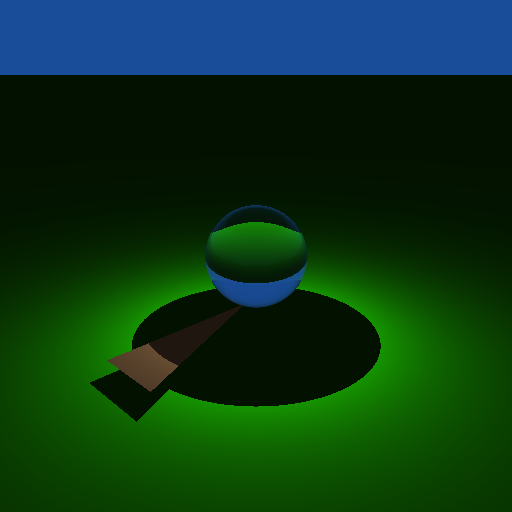
\includegraphics[width = \textwidth]{./Worksheet8/transparent_fresnel.png}\\
				\textit{R computed using fresnel equations}\\
			\end{center}
		\end{minipage}
		\hspace{0.05\linewidth}
		\begin{minipage}[b]{0.40\linewidth}
			\begin{center}
				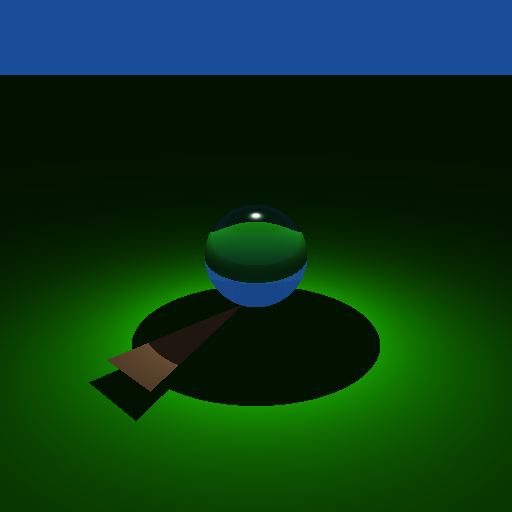
\includegraphics[width = \textwidth]{./Worksheet8/r01.png}\\
				\textit{R = 0.1 (kept constant)}
			\end{center}
		\end{minipage}
	\end{center}
	
	The difference is very subtle but we can see a small blue highlight on top of the sphere. This is due to the great importance of reflection at this angle. We can also see a gradient effect in the upper blue part at the bottom of the sphere where we have both sky refraction and shadow reflection. In the adaptive $R$ case we can see the evolution of this coefficient with a more blurry limit between these two zones at the center of the sphere (more refraction due to smaller angle).\\
	
	
	
	The code in	\textbf{Glossy.cpp} and \textbf{ParticleTracer.cpp} was already supporting this implementation, using the returned $R$ parameter of \textit{trace\_refracted}:
	\begin{lstlisting}
	float3 Glossy::shade(const Ray& r, HitInfo& hit, bool emit) const
	{
		if(hit.trace_depth >= max_depth)
		return make_float3(0.0f);
		
		float R;
		Ray reflected, refracted;
		HitInfo hit_reflected, hit_refracted;
		tracer->trace_reflected(r, hit, reflected, hit_reflected);
		tracer->trace_refracted(r, hit, refracted, hit_refracted, R);
		
		return R*shade_new_ray(reflected, hit_reflected) + (1.0f - R)*shade_new_ray(refracted, hit_refracted) + Phong::shade(r, hit, emit);
	}
	\end{lstlisting}
	
	\begin{lstlisting}
	void ParticleTracer::trace_particle(const Light* light, const unsigned int caustics_done)
	{
		if(caustics_done)
		return;
		
		// Shoot a particle from the sampled source
		Ray r;
		HitInfo hit;
		float3 Phi;
		if (!light->emit(r, hit, Phi)) {
			// If no hit at all
			return;
		}
		
		// Forward from all specular surfaces
		while(scene->is_specular(hit.material) && hit.trace_depth < 500)
		{
			switch(hit.material->illum)
			{
				case 3:  // mirror materials
				{
					// Forward from mirror surfaces here
					Ray r_out;
					HitInfo hit_out;
					if (!trace_reflected(r, hit, r_out, hit_out)) {
						return;
					}
					r = r_out;
					hit = hit_out;
				}
				break;
				case 11: // absorbing volume
				case 12: // absorbing glossy volume
				{
					// Handle absorption here (Worksheet 8)
				}
				case 2:  // glossy materials
				case 4:  // transparent materials
				{
					// Forward from transparent surfaces here
					Ray r_out;
					HitInfo hit_out;
					
					// Russian roulette to choose between reflection and refraction
					float P;
					trace_refracted(r, hit, r_out, hit_out, P);
					if (mt_random() < P) {
						hit_out.has_hit = false;
						trace_reflected(r, hit, r_out, hit_out);
					}
					
					if (!hit_out.has_hit) {
						return;
					}
					
					r = r_out;
					hit = hit_out;
				}
				break;
				default:
				return;
			}
		}
		
		// Store in caustics map at first diffuse surface
		// Hint: When storing, the convention is that the photon direction
		//       should point back toward where the photon came from.
		if (hit.trace_depth > 0)
		caustics.store(Phi, hit.position, -r.direction);
	}	
	\end{lstlisting}
	
	We can then compare the renderings of the default scene between $R$ as kept constant and computed using the fresnel equations, but the difference is again very subtle (however we can see the caustic reflexion at the top of the sphere):
	
	\begin{center}
		\begin{minipage}[b]{0.40\linewidth}
			\begin{center}
				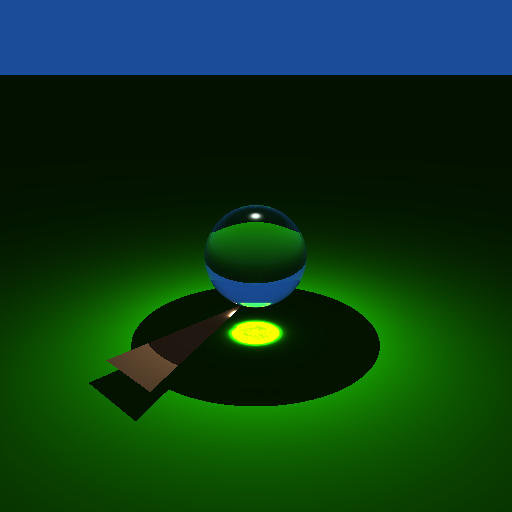
\includegraphics[width = \textwidth]{./Worksheet8/withcaustics.png}\\
				\textit{Glossy shader with caustics (R computed using fresnel equations)}\\
			\end{center}
		\end{minipage}
		\hspace{0.05\linewidth}
		\begin{minipage}[b]{0.40\linewidth}
			\begin{center}
				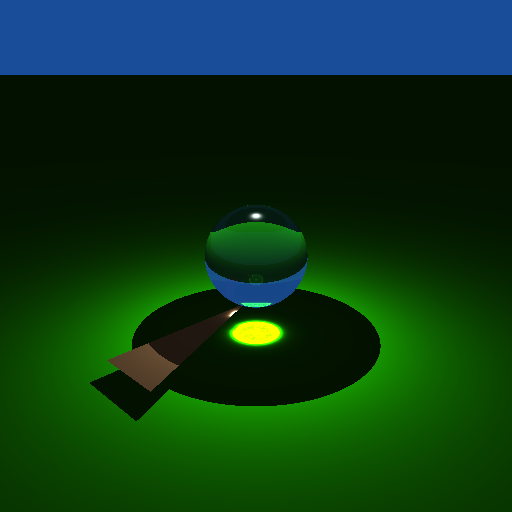
\includegraphics[width = \textwidth]{./Worksheet7/causticsandillumination.png}\\
				\textit{Glossy shader with caustics (R = 0.1, kept constant)}\\
			\end{center}
		\end{minipage}
	\end{center}
	
	\begin{center}
		\begin{center}
		\begin{minipage}[b]{0.40\linewidth}
			\begin{center}
				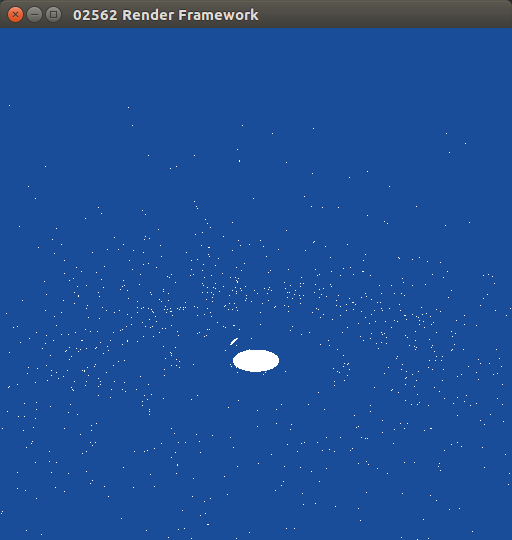
\includegraphics[width = \textwidth]{./Worksheet8/causticdots.png}\\
				\textit{Caustics map as white dots}\\
			\end{center}
		\end{minipage}
	\end{center}
	\end{center}
	
	\subsection{Absorption}
	Implementation of absorption in transparent materials in \textbf{Volume.cpp}:
	
	\begin{lstlisting}
	float3 Volume::shade(const Ray& r, HitInfo& hit, bool emit) const
	{
		// If inside the volume, Find the direct transmission through the volume by using
		// the transmittance to modify the result from the Transparent shader.
		// If inside the ray going out and the material normal (pointing outwards) are pointing in the same direction
		// (same hemisphere)
		if (dot(r.direction, hit.geometric_normal) > 0) {
			return get_transmittance(hit) * Transparent::shade(r, hit, emit);
		}
		return Transparent::shade(r, hit, emit);
	}
	\end{lstlisting}
	
	\begin{lstlisting}
	float3 Volume::get_transmittance(const HitInfo& hit) const
	{
		if(hit.material)
		{
			// Compute and return the transmittance using the diffuse reflectance of the material.
			float3 rho_d = make_float3(hit.material->diffuse[0], hit.material->diffuse[1], hit.material->diffuse[2]);
			float3 rho_d_corrected = make_float3(fmax(rho_d.x, 1e-5), fmax(rho_d.y, 1e-5), fmax(rho_d.z, 1e-5));
			float3 absorption = 1/rho_d_corrected - 1;
			return make_float3(exp(-absorption.x*hit.dist), exp(-absorption.y*hit.dist), exp(-absorption.z*hit.dist));
		}
		//No material, full transmission
		return make_float3(1.0f);
	}
	\end{lstlisting}
	
	We then implement the glossy shader including absorption. To do this we use the Phong specular component (we exclude its diffusive component to use the glass absorption properties) along with the glossy shader computations. Finally we use the transmittance coefficient to scale the radiance if a material was traversed:
	\textbf{GlossyVolume.cpp}:
	
	\begin{lstlisting}
	float3 GlossyVolume::shade(const Ray& r, HitInfo& hit, bool emit) const
	{
		float3 rho_s = get_specular(hit);
		float s = get_shininess(hit);
		
		float3 wi, wo, wr, Li;
		float3 Lr = make_float3(0.0);
		for (int i = 0; i < lights.size(); i++) {
			Light *light = lights[i];
			if (light->sample(hit.position, wi, Li)) {
				// Not in shadows, we add this light participation
				wr = normalize(reflect(-wi, hit.shading_normal));
				wo = normalize(-r.direction);
				
				// Compute phong for this light
				Li = make_float3(fmax(dot(wi, hit.shading_normal), 0));
				
				float dotproduct = dot(wo, wr);
				dotproduct = fmax(dotproduct, 0);
				
				Li *= rho_s*(s + 2)*pow(dotproduct, s)*M_1_PIf/2;
				Lr += Li;
			}
		}
		
		if(hit.trace_depth >= max_depth)
		return make_float3(0.0f);
		
		float R;
		Ray reflected, refracted;
		HitInfo hit_reflected, hit_refracted;
		tracer->trace_reflected(r, hit, reflected, hit_reflected);
		tracer->trace_refracted(r, hit, refracted, hit_refracted, R);
		
		float3 res = R*shade_new_ray(reflected, hit_reflected) + (1.0f - R)*shade_new_ray(refracted, hit_refracted) + Lr;
		
		if (dot(r.direction, hit.geometric_normal) > 0) {
			return get_transmittance(hit) * res;
		}
		
		return res;
	}
	\end{lstlisting}
	
	The only missing part of our model is implementing this absorption for the caustics, this is done in \textbf{ParticleTracer.cpp}:
	
	\begin{lstlisting}
	float3 ParticleTracer::get_transmittance(const HitInfo& hit) const
	{
		if(hit.material)
		{
			// Compute and return the transmittance using the diffuse reflectance of the material.
			// Diffuse reflectance rho_d does not make sense for a specular material, so we can use
			// this material property as an absorption coefficient. Since absorption has an effect
			// opposite that of reflection, using 1/rho_d-1 makes it more intuitive for the user.
			float3 rho_d = make_float3(hit.material->diffuse[0], hit.material->diffuse[1], hit.material->diffuse[2]);
			float3 rho_d_corrected = make_float3(fmax(rho_d.x, 1e-5), fmax(rho_d.y, 1e-5), fmax(rho_d.z, 1e-5));
			float3 absorption = 1/rho_d_corrected - 1;
			return make_float3(exp(-absorption.x*hit.dist), exp(-absorption.y*hit.dist), exp(-absorption.z*hit.dist));
		}
		//No material, full transmission
		return make_float3(1.0f);
	}
	\end{lstlisting}
	
	\begin{lstlisting}
	void ParticleTracer::trace_particle(const Light* light, const unsigned int caustics_done)
	{
		if(caustics_done)
		return;
		
		// Shoot a particle from the sampled source
		Ray r;
		HitInfo hit;
		float3 Phi;
		if (!light->emit(r, hit, Phi)) {
			// If no hit at all
			return;
		}
		
		// Forward from all specular surfaces
		while(scene->is_specular(hit.material) && hit.trace_depth < 500)
		{
			switch(hit.material->illum)
			{
				case 3:  // mirror materials
				{
					// Forward from mirror surfaces here
					Ray r_out;
					HitInfo hit_out;
					if (!trace_reflected(r, hit, r_out, hit_out)) {
						return;
					}
					r = r_out;
					hit = hit_out;
				}
				break;
				case 11: // absorbing volume
				case 12: // absorbing glossy volume
				{
					Phi = Phi*get_transmittance(hit);
				}
				case 2:  // glossy materials
				case 4:  // transparent materials
				{
					// Forward from transparent surfaces here
					Ray r_out;
					HitInfo hit_out;
					
					// Russian roulette to choose between reflection and refraction
					float P;
					trace_refracted(r, hit, r_out, hit_out, P);
					if (mt_random() < P) {
						hit_out.has_hit = false;
						trace_reflected(r, hit, r_out, hit_out);
					}
					
					if (!hit_out.has_hit) {
						return;
					}
					
					r = r_out;
					hit = hit_out;
				}
				break;
				default:
				return;
			}
		}
		if (hit.trace_depth > 0)
		caustics.store(Phi, hit.position, -r.direction);
	}
	\end{lstlisting}
	
	We can visualize the results, using different transmission parameters for $K_d(r, g, b)$. All the images below had gamma increased once to show bigger contrasts:
	
	\begin{center}
		\begin{minipage}[b]{0.40\linewidth}
			\begin{center}
				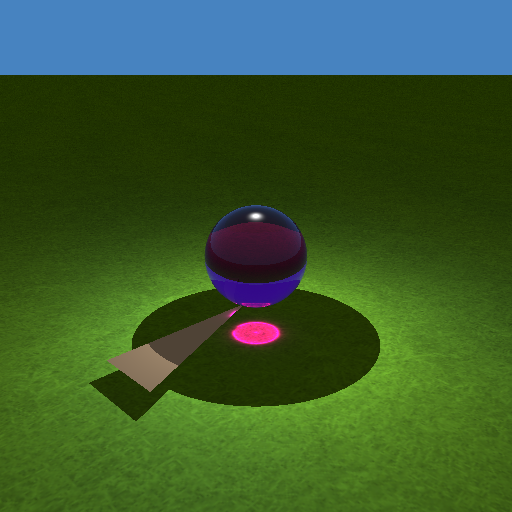
\includegraphics[width = \textwidth]{./Worksheet8/pinkball.png}\\
				\textit{Purple couloured glass sphere\\Kd = 0.9, 0.1, 0.5}\\
			\end{center}
		\end{minipage}
		\hspace{0.05\linewidth}
		\begin{minipage}[b]{0.40\linewidth}
			\begin{center}
				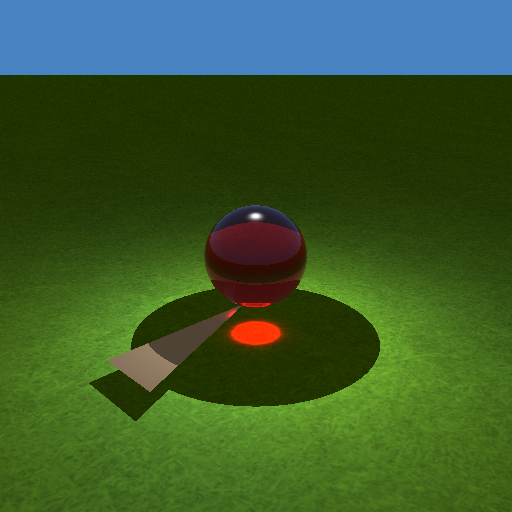
\includegraphics[width = \textwidth]{./Worksheet8/redball.png}\\
				\textit{Red couloured glass sphere\\Kd = 0.9, 0.1, 0.1}\\
			\end{center}
		\end{minipage}
	\end{center}
	
	
	
\end{document}
% Fin du document LaTeX
